%%%%%%%%%%%%%%%%%%%%%%%%%%%%%%%%%%%%%%%%%
% Short Sectioned Assignment
% LaTeX Template
% Version 1.0 (5/5/12)
%
% This template has been downloaded from:
% http://www.LaTeXTemplates.com
%
% Original author:
% Frits Wenneker (http://www.howtotex.com)
%
% License:
% CC BY-NC-SA 3.0 (http://creativecommons.org/licenses/by-nc-sa/3.0/)
%
%%%%%%%%%%%%%%%%%%%%%%%%%%%%%%%%%%%%%%%%%

%----------------------------------------------------------------------------------------
%	PACKAGES AND OTHER DOCUMENT CONFIGURATIONS
%----------------------------------------------------------------------------------------

\documentclass[paper=a4, fontsize=11pt]{scrartcl} % A4 paper and 11pt font size

\usepackage[T1]{fontenc} % Use 8-bit encoding that has 256 glyphs
\usepackage{fourier} % Use the Adobe Utopia font for the document - comment this line to return to the LaTeX default
\usepackage[english]{babel} % English language/hyphenation
\usepackage{amsmath,amsfonts,amsthm} % Math packages

\usepackage{graphicx}

\usepackage{sectsty} % Allows customizing section commands
\allsectionsfont{\centering \normalfont\scshape} % Make all sections centered, the default font and small caps

\usepackage{subcaption}
\usepackage{pdfpages}
\usepackage{float}
\usepackage{url}
\usepackage{listings}
\usepackage[toc,page]{appendix}

\usepackage{fancyhdr} % Custom headers and footers
\pagestyle{fancyplain} % Makes all pages in the document conform to the custom headers and footers
\fancyhead{} % No page header - if you want one, create it in the same way as the footers below
\fancyfoot[L]{} % Empty left footer
\fancyfoot[C]{} % Empty center footer
\fancyfoot[R]{\thepage} % Page numbering for right footer
\renewcommand{\headrulewidth}{0pt} % Remove header underlines
\renewcommand{\footrulewidth}{0pt} % Remove footer underlines
\setlength{\headheight}{13.6pt} % Customize the height of the header

\numberwithin{equation}{section} % Number equations within sections (i.e. 1.1, 1.2, 2.1, 2.2 instead of 1, 2, 3, 4)
\numberwithin{figure}{section} % Number figures within sections (i.e. 1.1, 1.2, 2.1, 2.2 instead of 1, 2, 3, 4)
\numberwithin{table}{section} % Number tables within sections (i.e. 1.1, 1.2, 2.1, 2.2 instead of 1, 2, 3, 4)

\setlength\parindent{0pt} % Removes all indentation from paragraphs - comment this line for an assignment with lots of text

%----------------------------------------------------------------------------------------
%	TITLE SECTION
%----------------------------------------------------------------------------------------

\newcommand{\horrule}[1]{\rule{\linewidth}{#1}} % Create horizontal rule command with 1 argument of height

\title{	
\normalfont \normalsize 
\textsc{Bonn-Rhein-Sieg University of Applied Sciences} \\ [25pt] % Your university, school and/or department name(s)
\horrule{0.5pt} \\[0.4cm] % Thin top horizontal rule
\huge Scientific Experimentation and Evaluation\\
- Task 5 : Motion Model - \\ 
% The assignment title
\horrule{2pt} \\[0.5cm] % Thick bottom horizontal rule
}

\author{Mazin Eltayeb, Bastian Lang} % Your name

\date{\normalsize\today} % Today's date or a custom date

\begin{document}

\maketitle % Print the title

\tableofcontents
\newpage

\section{Abstract}
This report describes how we solved the task of determining the parameters of the motion model for our LEGO NXT robot. We will describe the experiments we performed, the preprocessing of the data and the way we computed the parameters. The results and the code can be found in the Appendix.

\section{Experiments}
In our experiments we commanded the robot to do two different sized left circles and two different sized right circles. All movements have been performed with different velocities. The values can be seen in table \ref{table:commands}. The motion trajectories can be seen in the figures in Appendix \ref{sec:plots}.



\section{Obtaining Alphas}
To calculate the alphas we first needed to pre-process our obtained log data. The entries needed to be cropped by the first and last 450 entries because those weren't part of the actual motion.
For each different kind of motion we applied Thrun's algorithm to calculate $\hat{v}$, $\hat{w}$ and $\hat{\gamma}$ and then computed their means and standard deviations.
Using pseudo inverse we then used to acquire the alpha values.

\begin{appendix}
\section{Commands}
\begin{table}[]
\centering
\caption{Motor Commands}
\label{table:commands}
\begin{tabular}{lllll}
Log no. & Right wheel turns & Right wheel power & Left Wheel turns & Left wheel power \\
1       & 200               & 100               & 100              & 50               \\
2       & 200               & 100               & 50               & 25               \\
3       & 100               & 50                & 200              & 100              \\
4       & 50                & 25                & 200              & 100             
\end{tabular}
\end{table}

\section{Results}
\begin{table}[]
\centering
\caption{Obtained Values From Each Log File}
\label{table:logs}
\begin{tabular}[H]{llllll}
Log No & V in m/s & Omega in radiant/s  & Sigma1 & Sigma2     & Sigma3 \\
1      & 0.0582   & 2.2015e-04  & 0.2900 & 8.4868e-04 & 0.0101 \\
2      & -0.2020  & -0.0011    & 0.1514 & 0.0009     & 0.0125 \\
3      & -0.1432  & -0.0004    & 0.2666 & 0.0008     & 0.0109 \\
4      & -0.2472  & -0.0030    & 0.0630 & 0.0012     & 0.0131
\end{tabular}
\end{table}

\begin{table}[H]
\centering
\caption{Obtained Alphas}
\label{table:Alphas}
\begin{tabular}{ll}
Parameter & Value     \\
Alpha1    & 2.1242    \\
Alpha2    & -158.9048 \\
Alpha3    & 0.0063    \\
Alpha4    & -0.1271   \\
Alpha5    & 0.0864    \\
Alpha6    & -2.8262  
\end{tabular}
\end{table}

\section{Plots}
\label{sec:plots}

%% Log 1
\begin{figure}[H]
	\centering
	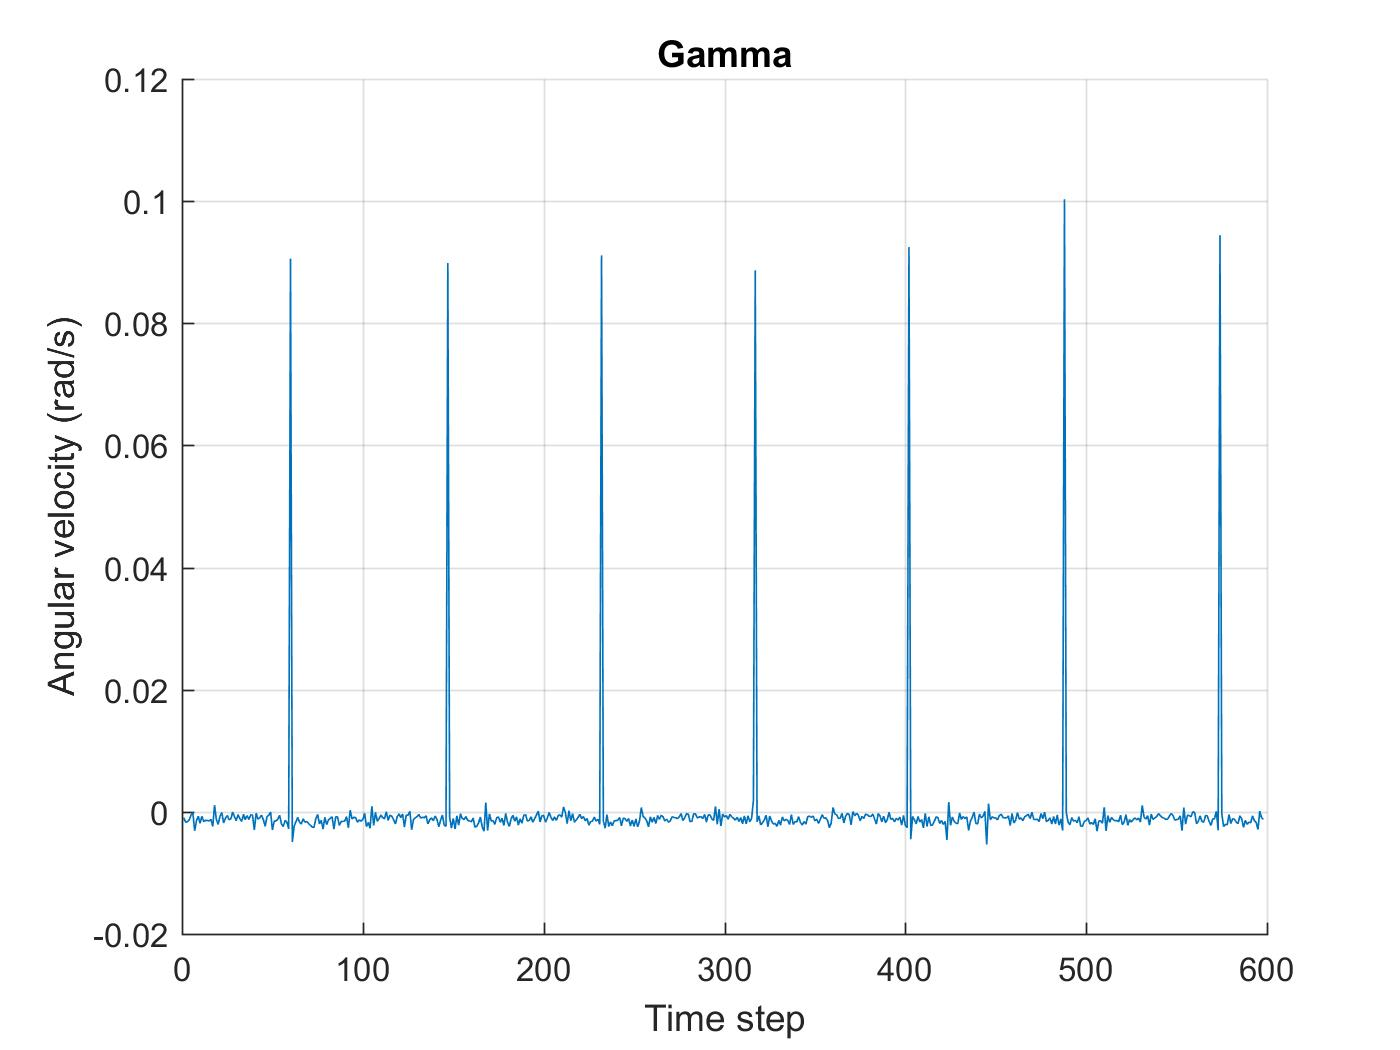
\includegraphics[width = 0.6\linewidth]{./figures/log1/gammaVsTime.jpg}
	\caption{log1:Gamma vs Time}
\end{figure}

\begin{figure}[H]
	\centering
	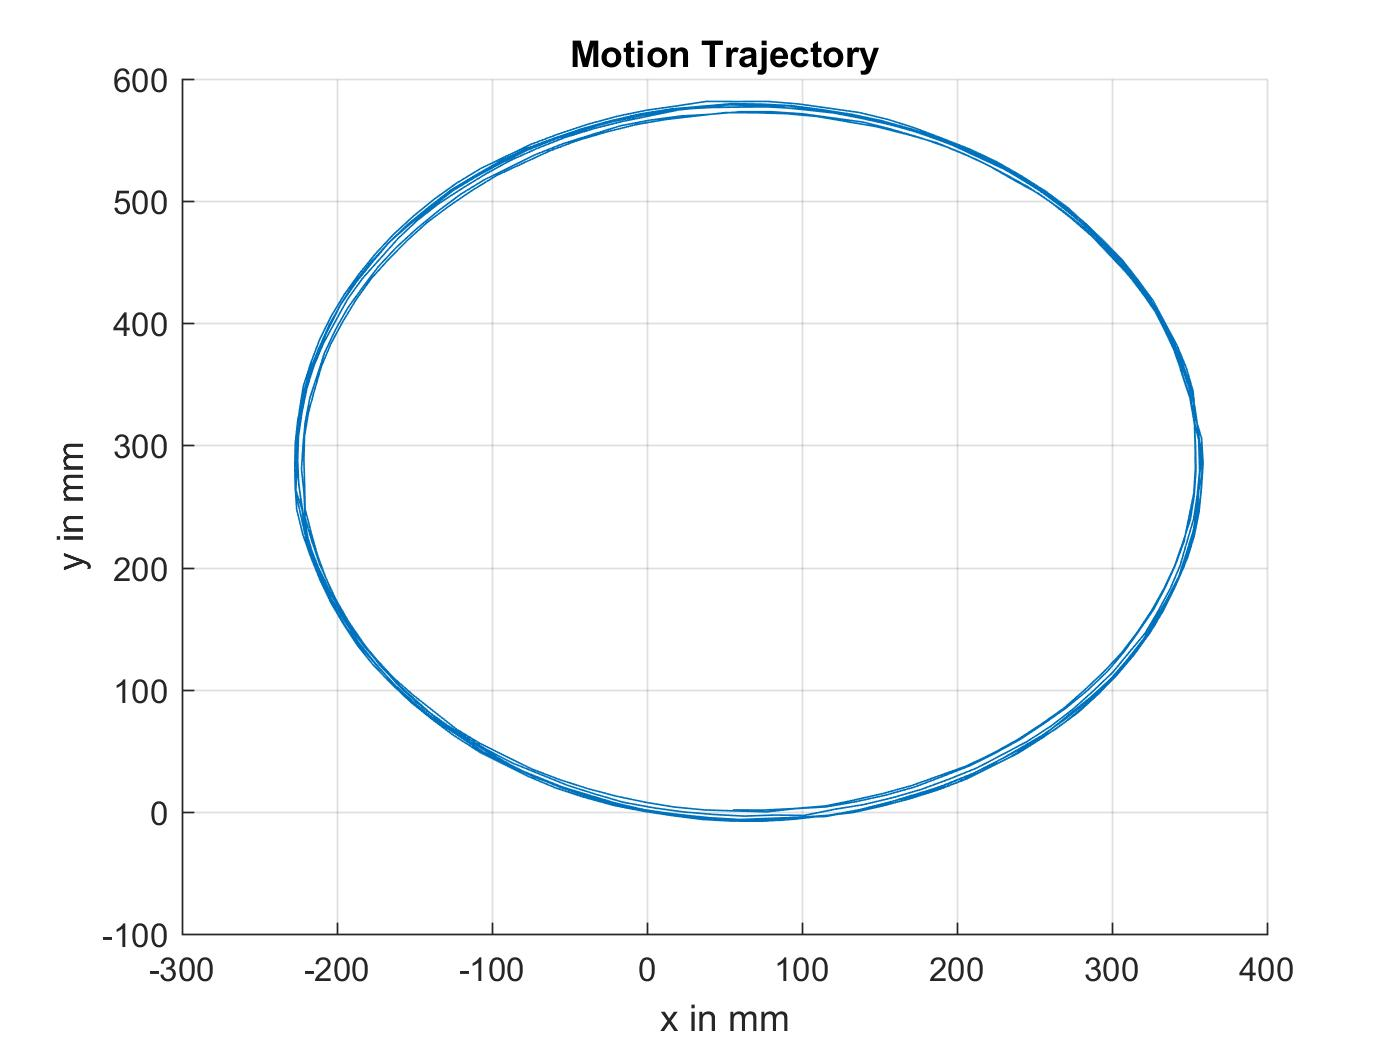
\includegraphics[width = 0.6\linewidth]{./figures/log1/motionTrajectory.jpg}
	\caption{log1:Motion Trajectory}
\end{figure}

\begin{figure}[H]
	\centering
	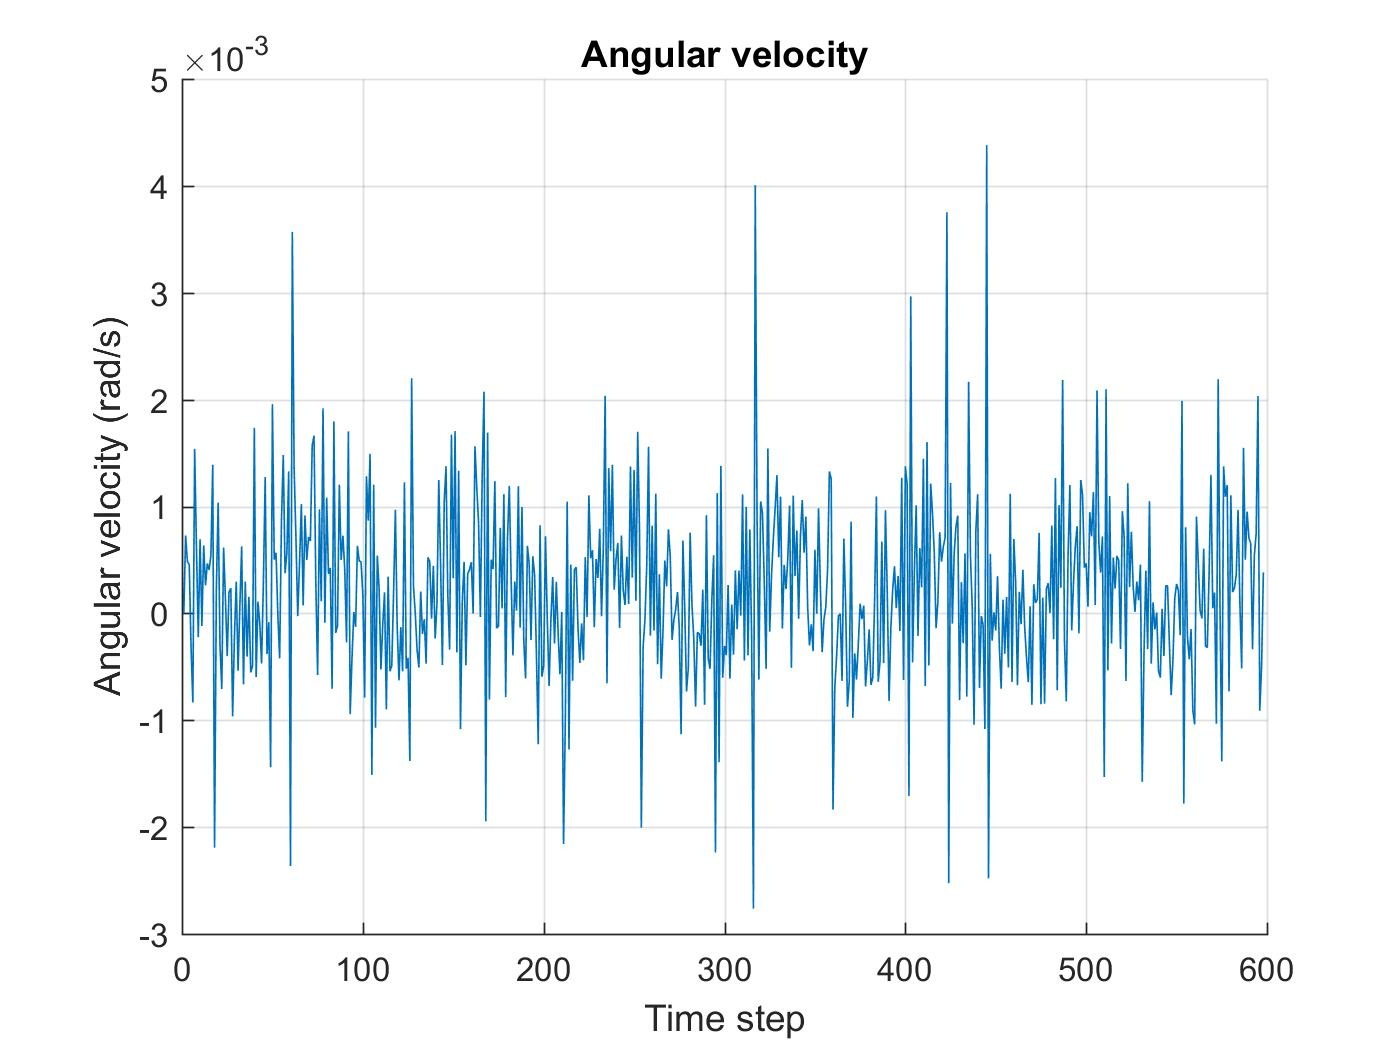
\includegraphics[width = 0.6\linewidth]{./figures/log1/omegaVsTime.jpg}
	\caption{log1:Omega vs Time}
\end{figure}

\begin{figure}[H]
	\centering
	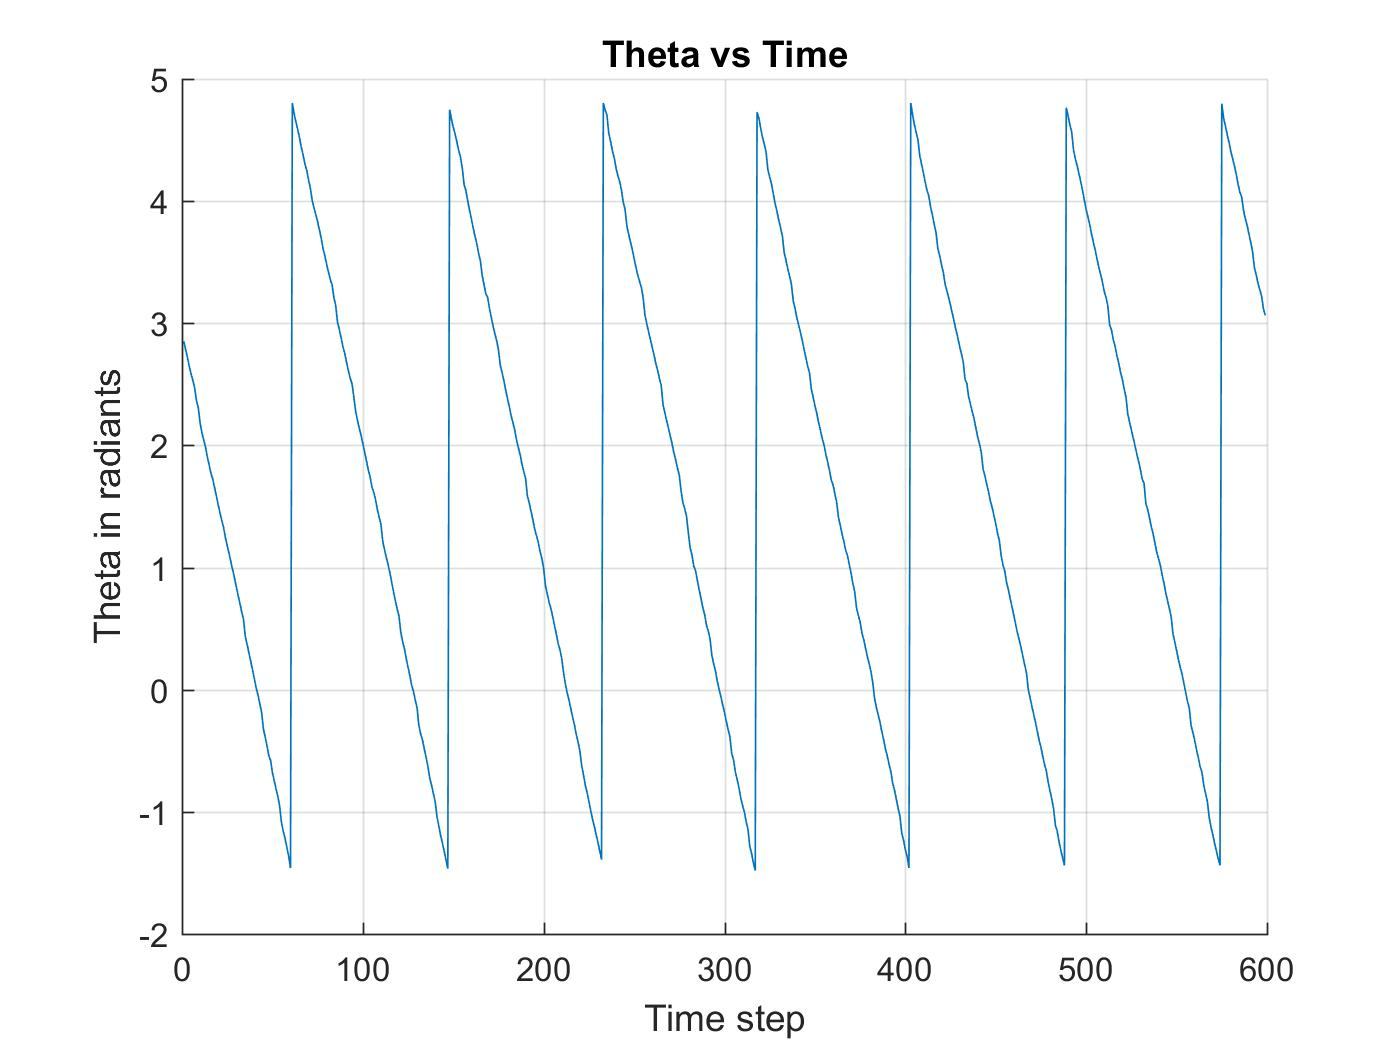
\includegraphics[width = 0.6\linewidth]{./figures/log1/thetaVsTime.jpg}
	\caption{log1:Theta vs Time}
\end{figure}

\begin{figure}[H]
	\centering
	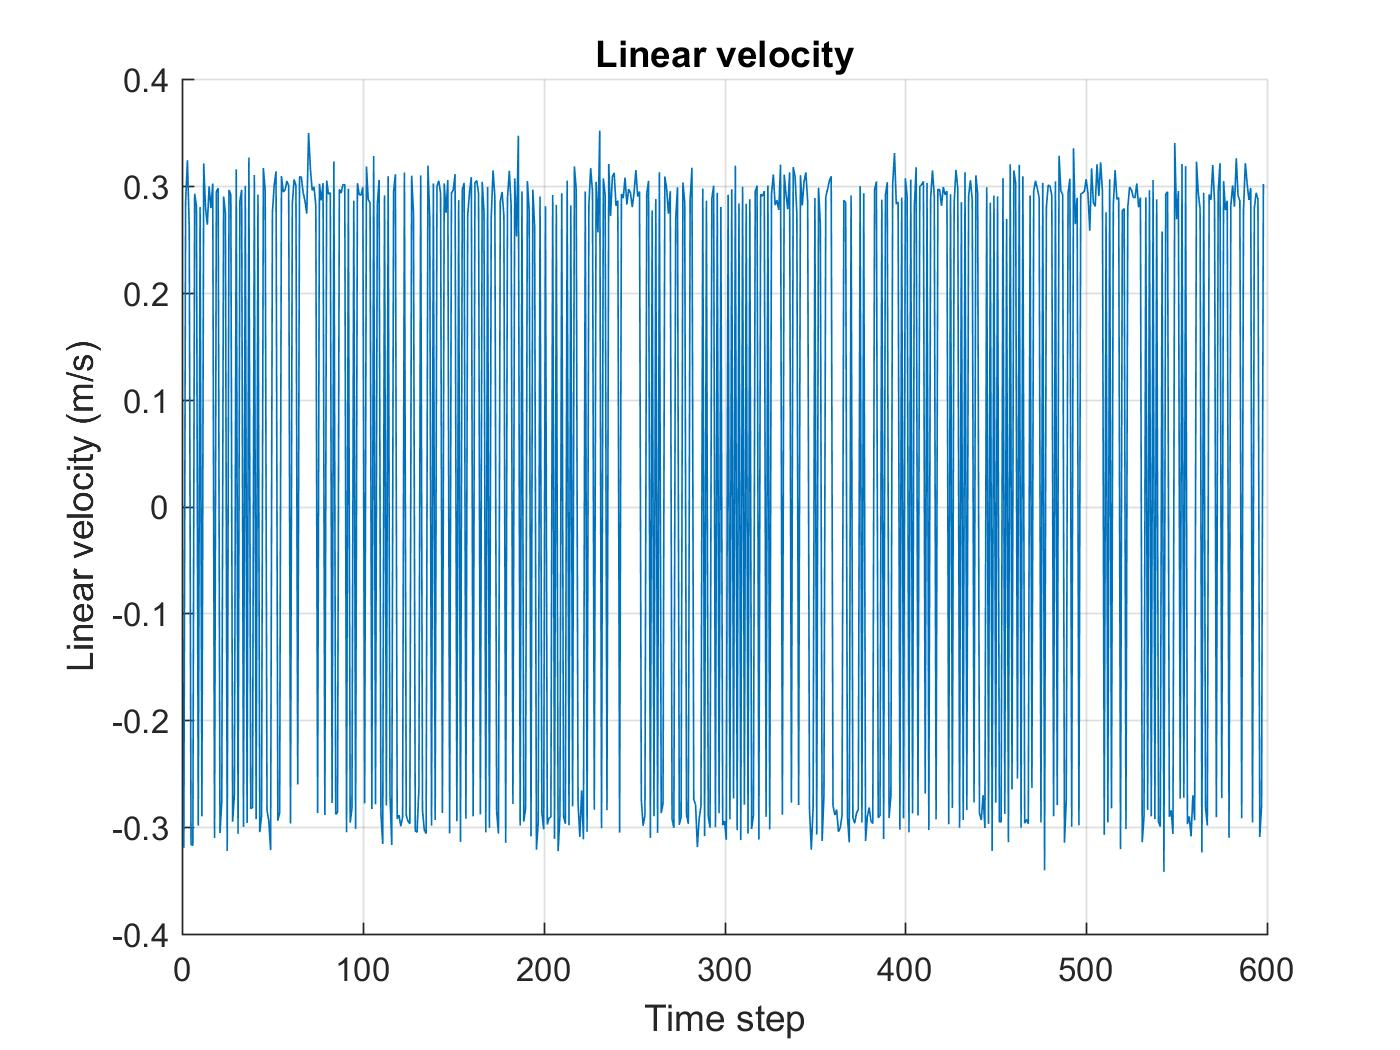
\includegraphics[width = 0.6\linewidth]{./figures/log1/vVsTime.jpg}
	\caption{log1:V vs Time}
\end{figure}

\begin{figure}[H]
	\centering
	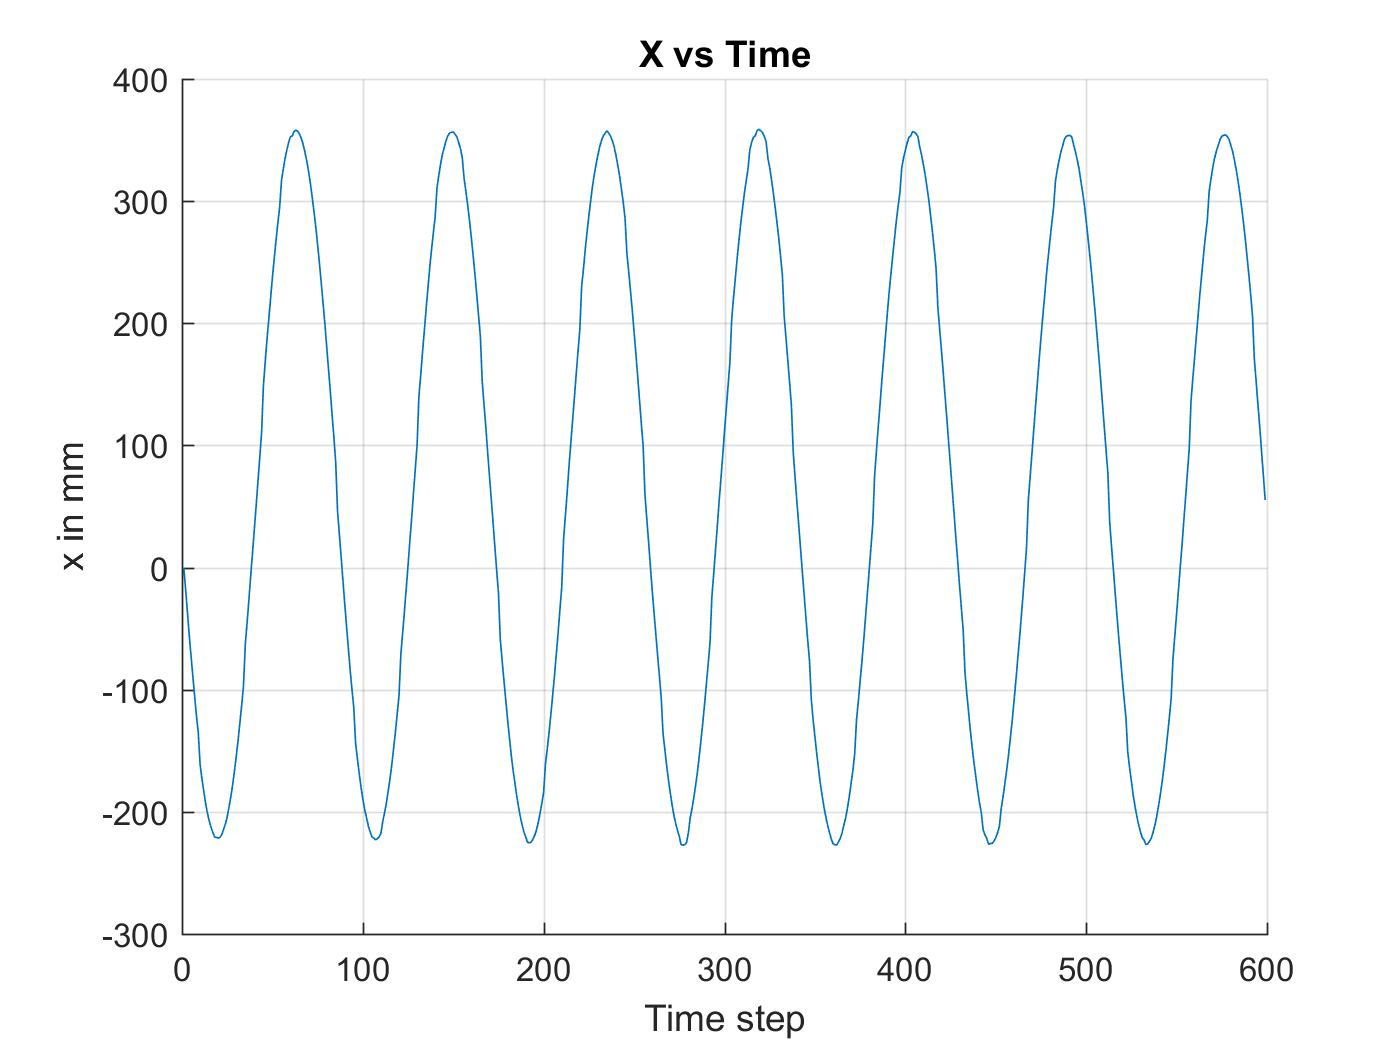
\includegraphics[width = 0.6\linewidth]{./figures/log1/xVsTime.jpg}
	\caption{log1:X vs Time}
\end{figure}

\begin{figure}[H]
	\centering
	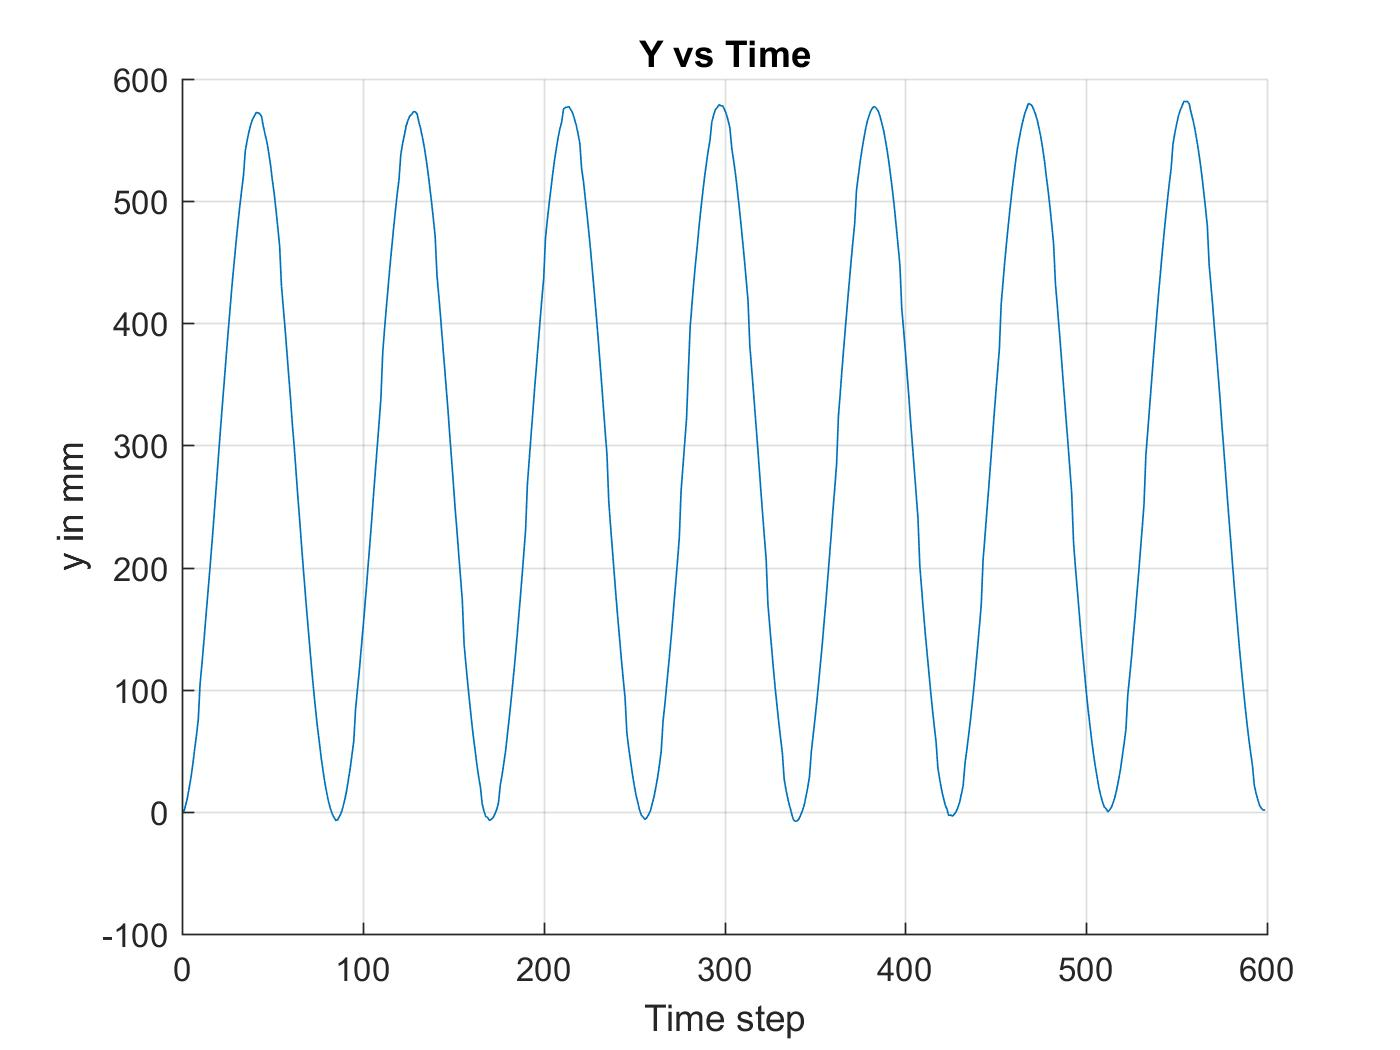
\includegraphics[width = 0.6\linewidth]{./figures/log1/yVsTime.jpg}
	\caption{log1:Y vs Time}
\end{figure}

%Log 2
\begin{figure}[H]
	\centering
	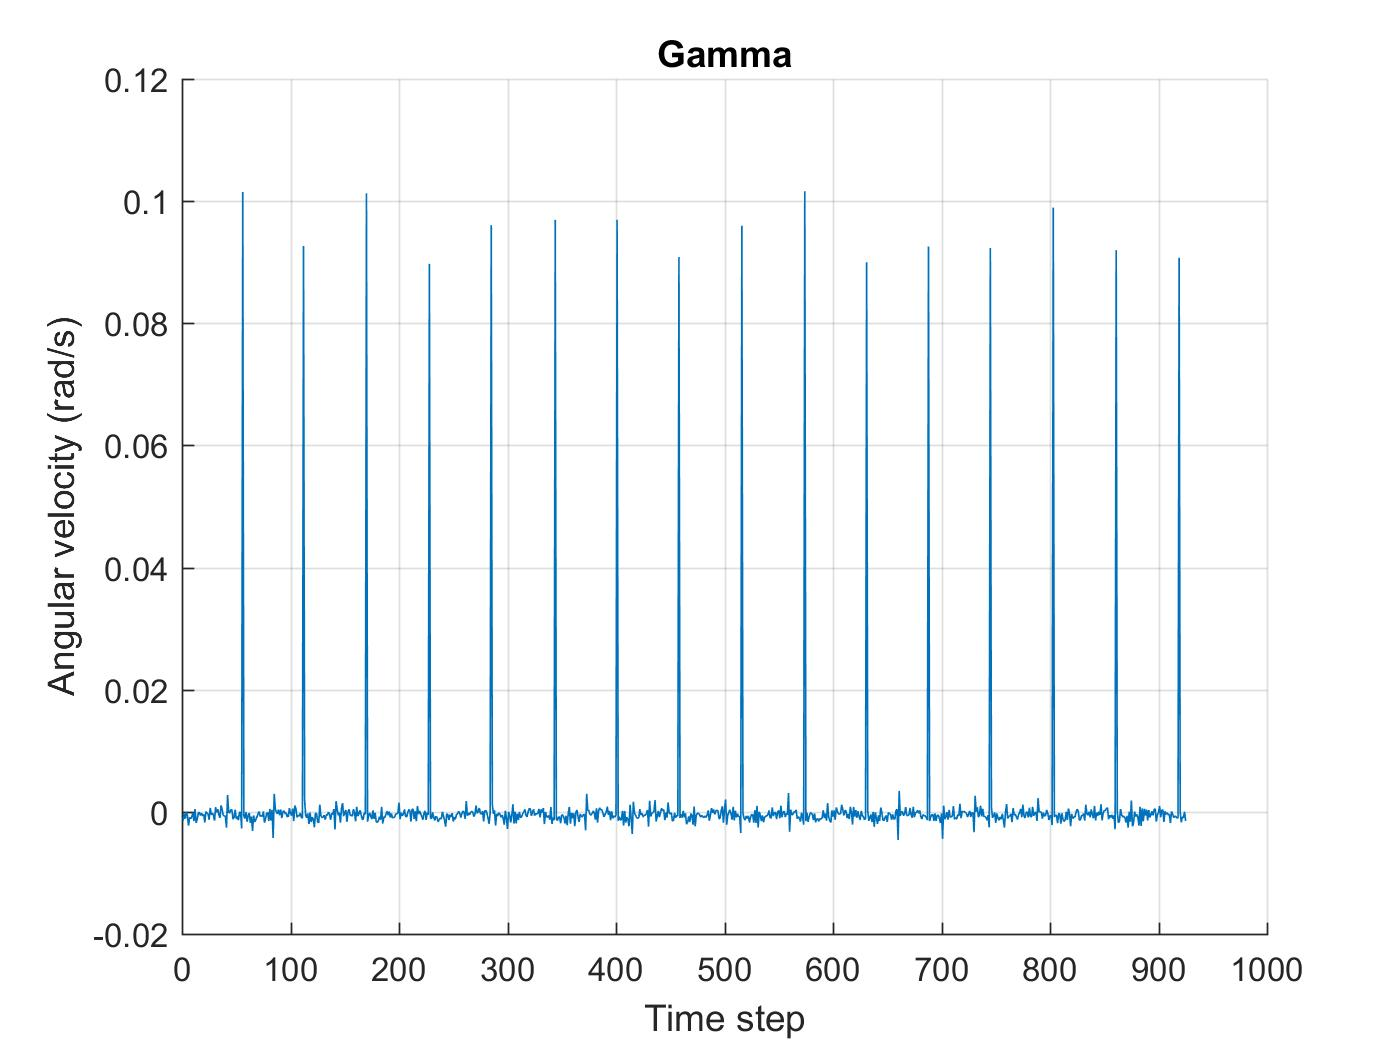
\includegraphics[width = 0.6\linewidth]{./figures/log2/gammaVsTime.jpg}
	\caption{log2:Gamma vs Time}
\end{figure}

\begin{figure}[H]
	\centering
	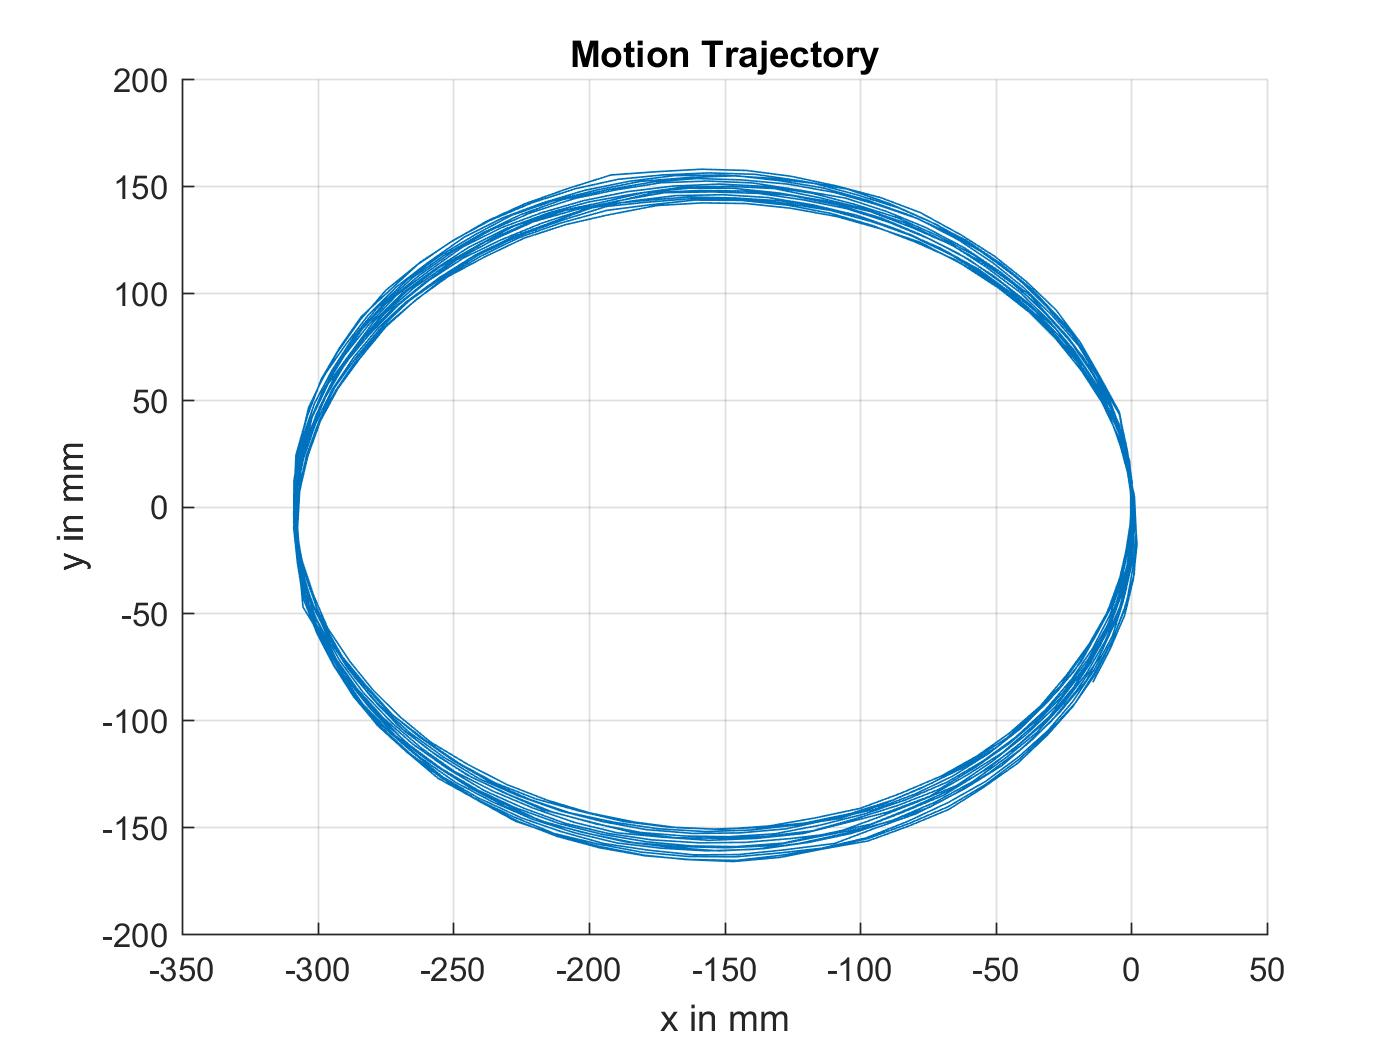
\includegraphics[width = 0.6\linewidth]{./figures/log2/motionTrajectory.jpg}
	\caption{log2:Motion Trajectory}
\end{figure}

\begin{figure}[H]
	\centering
	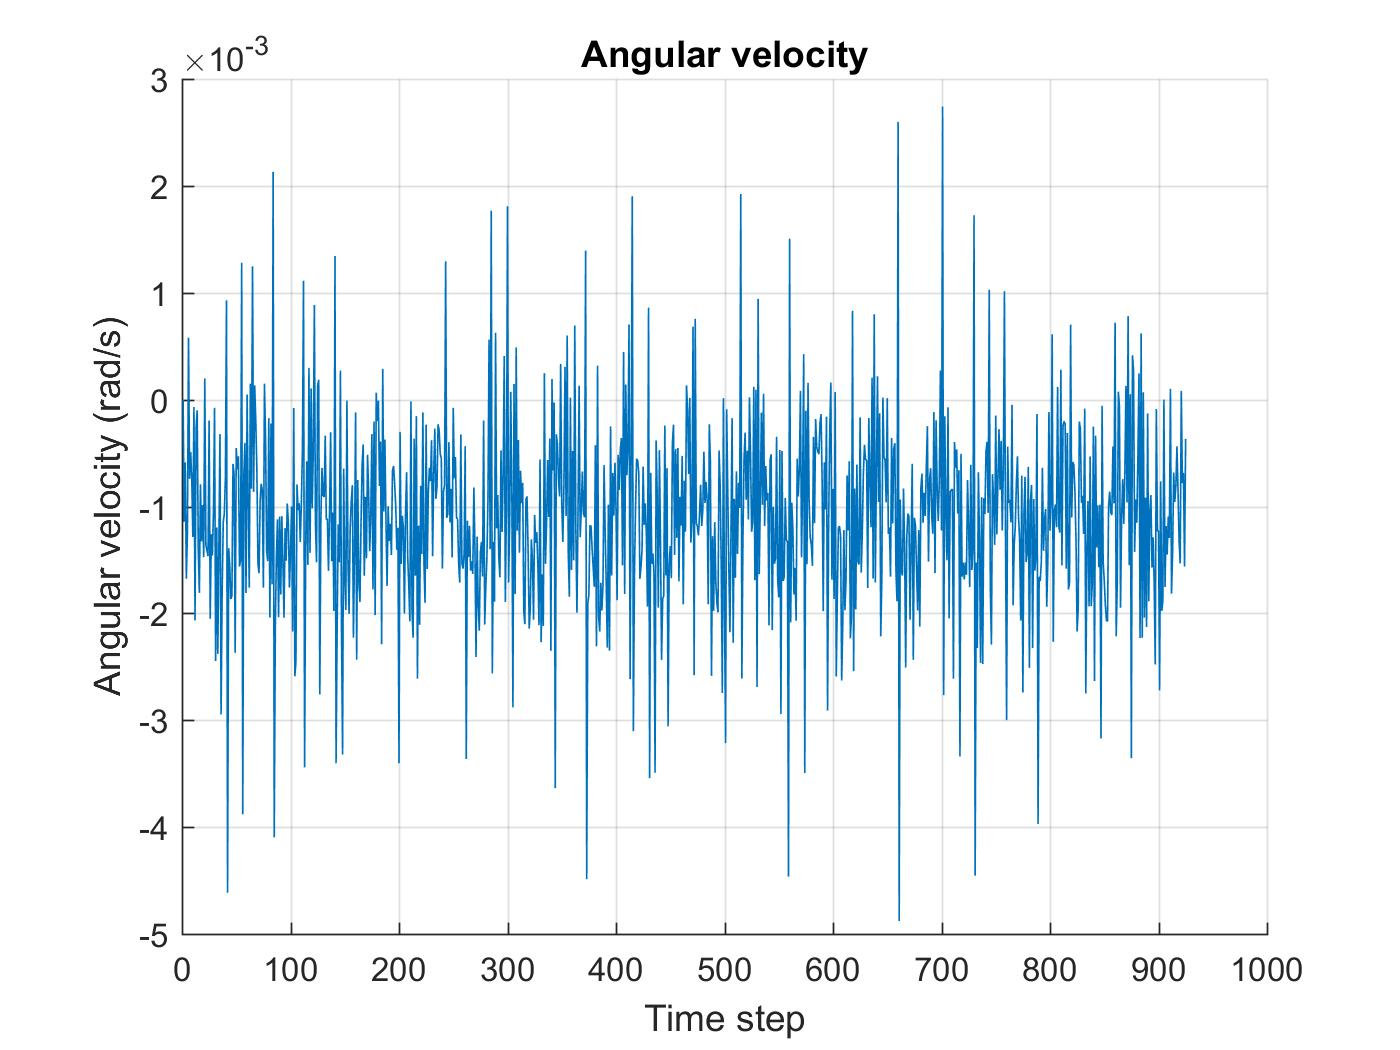
\includegraphics[width = 0.6\linewidth]{./figures/log2/omegaVsTime.jpg}
	\caption{log2:Omega vs Time}
\end{figure}

\begin{figure}[H]
	\centering
	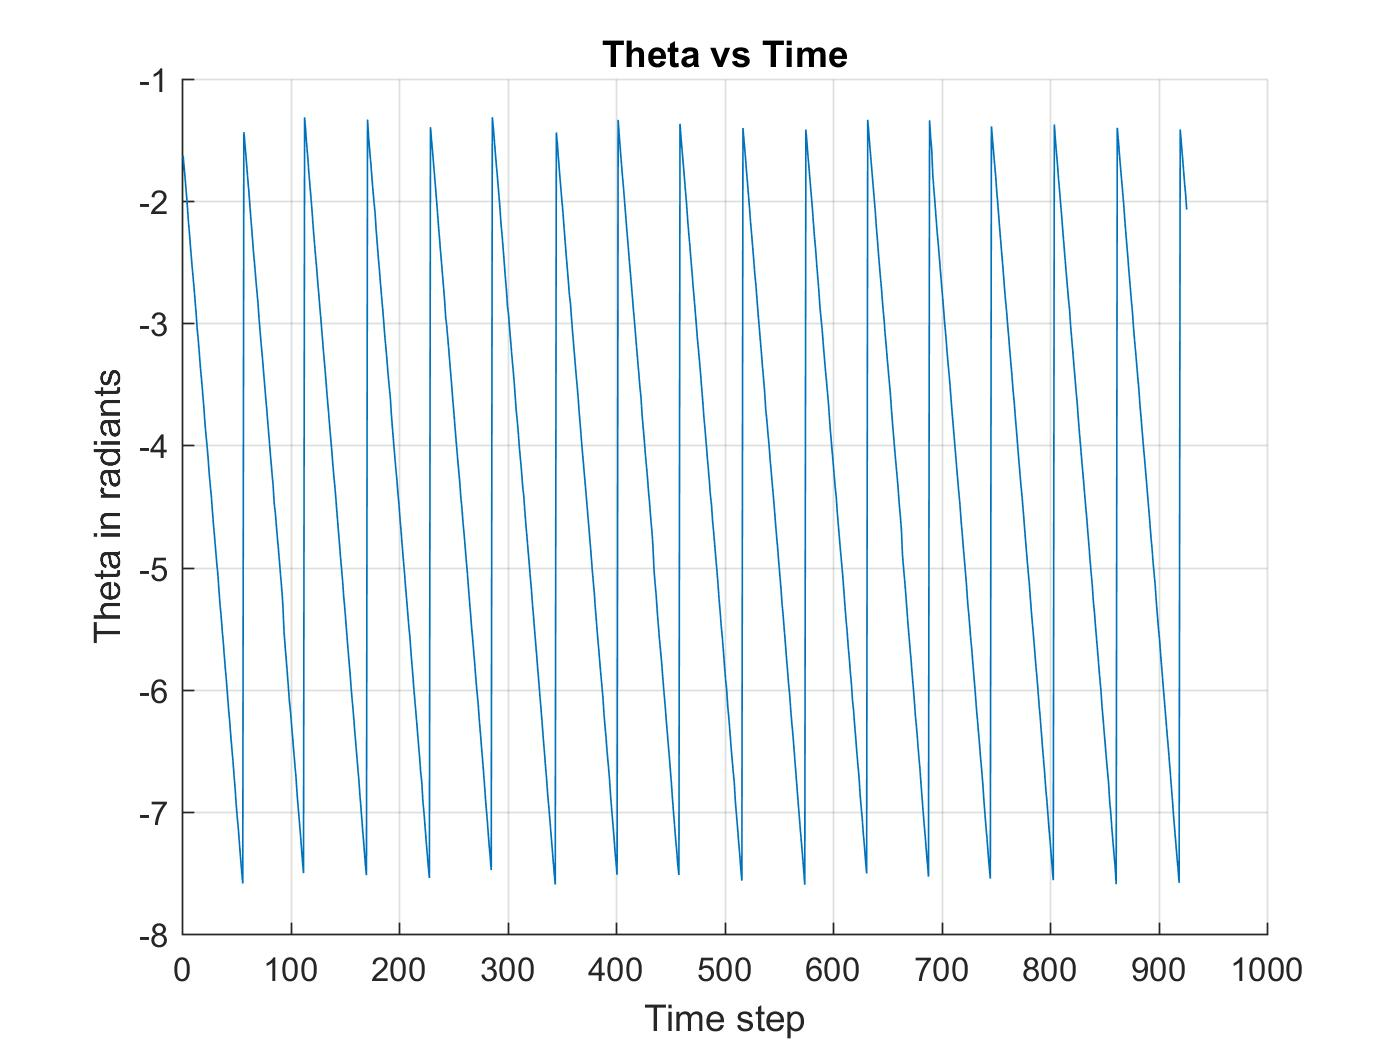
\includegraphics[width = 0.6\linewidth]{./figures/log2/thetaVsTime.jpg}
	\caption{log2:Theta vs Time}
\end{figure}

\begin{figure}[H]
	\centering
	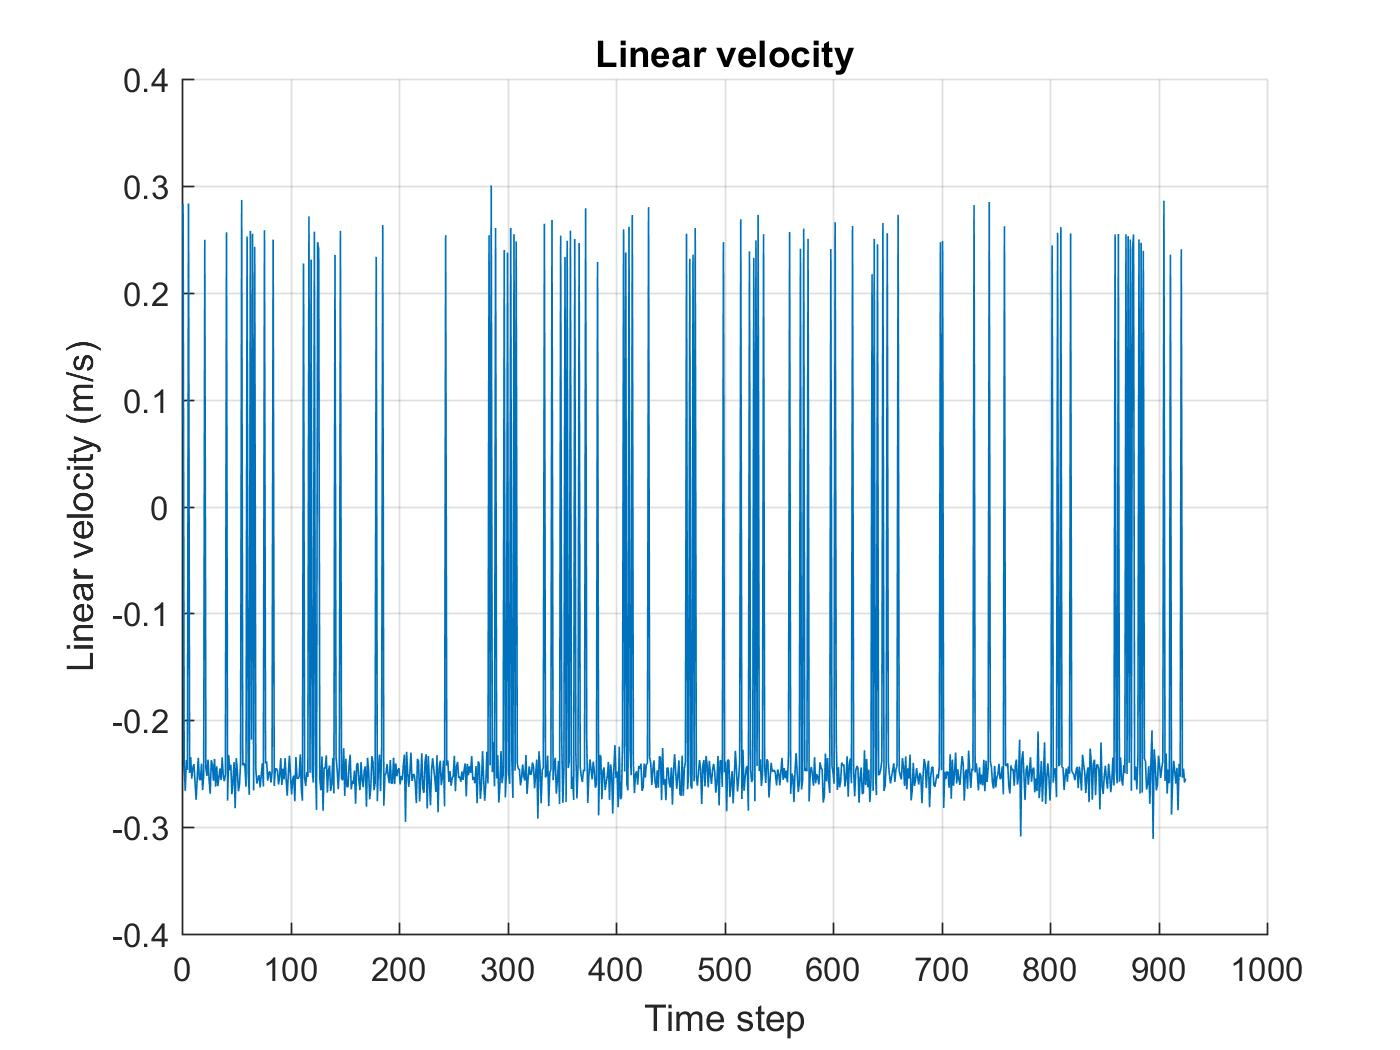
\includegraphics[width = 0.6\linewidth]{./figures/log2/vVsTime.jpg}
	\caption{log2:V vs Time}
\end{figure}

\begin{figure}[H]
	\centering
	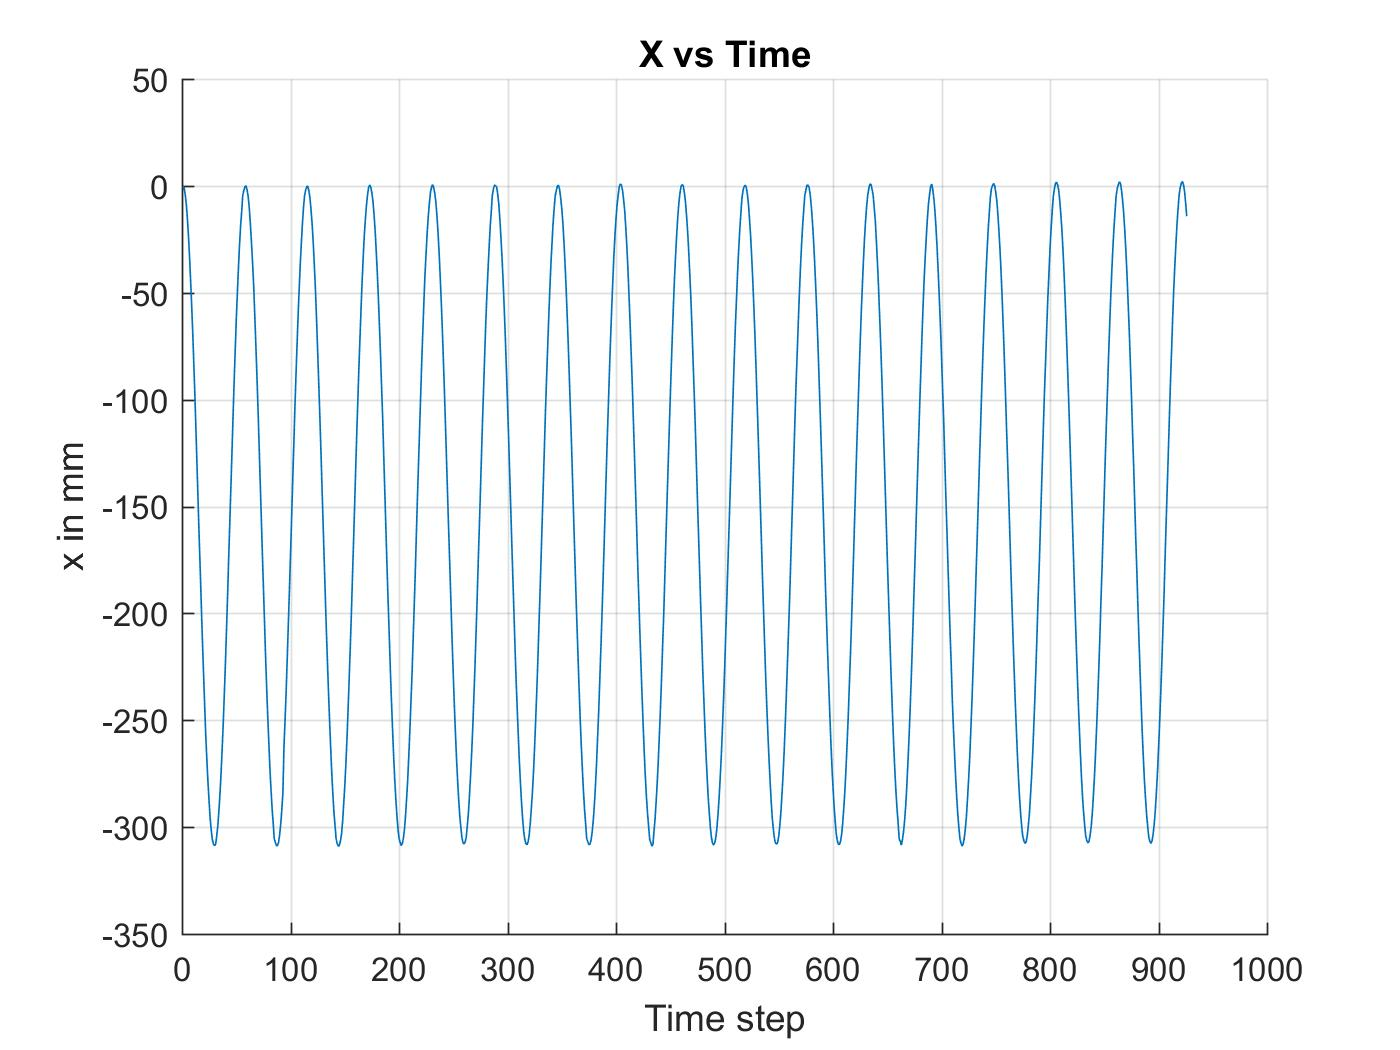
\includegraphics[width = 0.6\linewidth]{./figures/log2/xVsTime.jpg}
	\caption{log2:X vs Time}
\end{figure}

\begin{figure}[H]
	\centering
	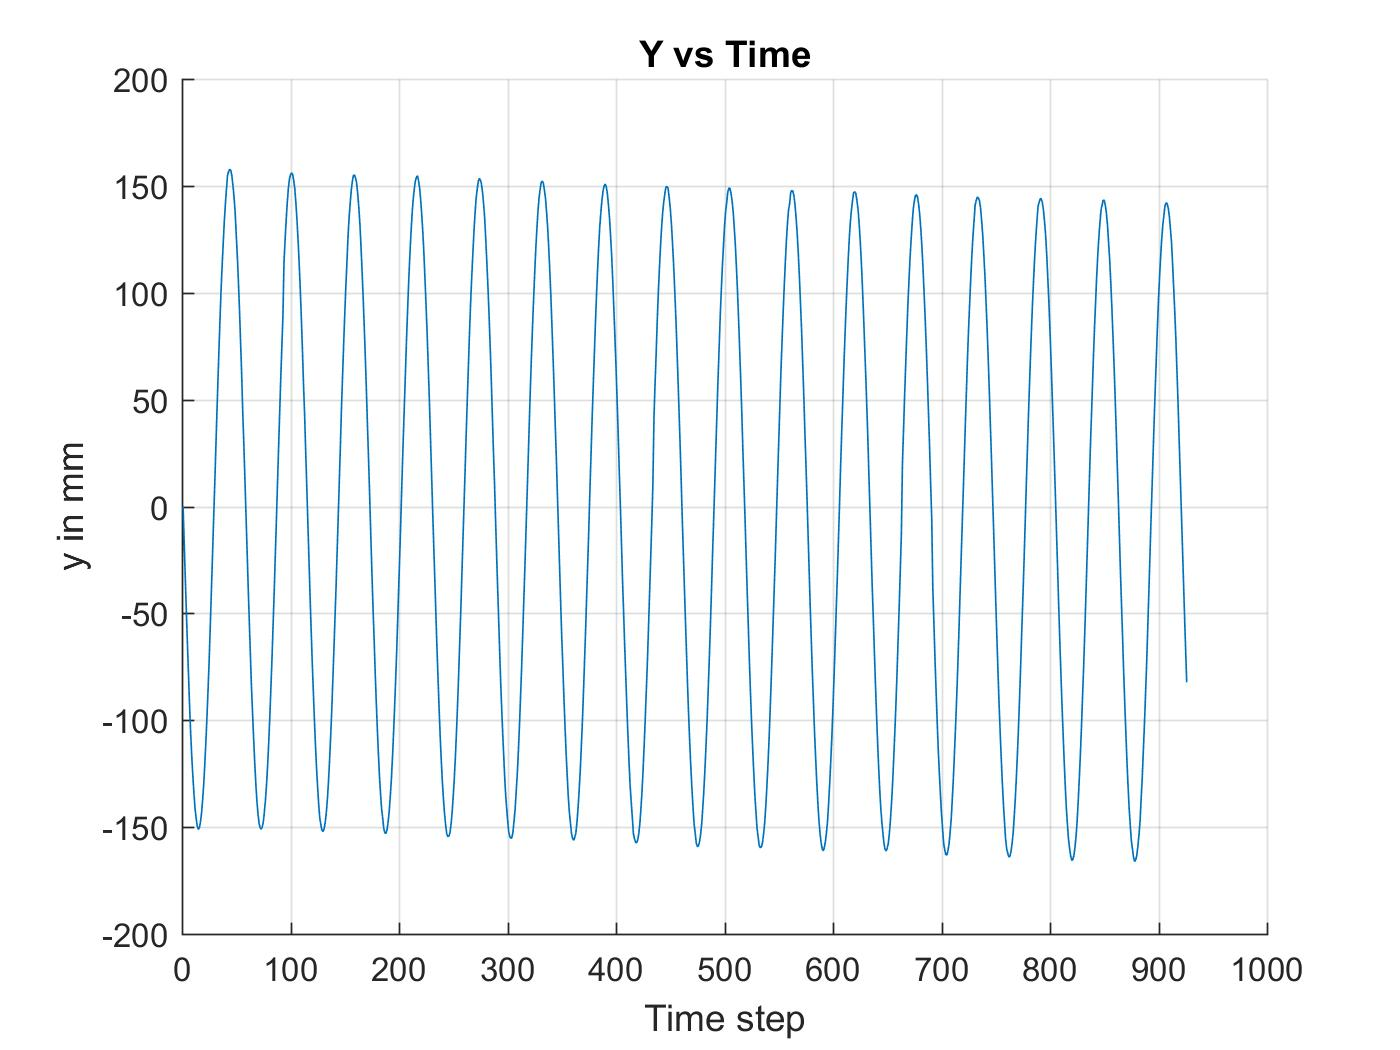
\includegraphics[width = 0.6\linewidth]{./figures/log2/yVsTime.jpg}
	\caption{log2:Y vs Time}
\end{figure}

%log 3
\begin{figure}[H]
	\centering
	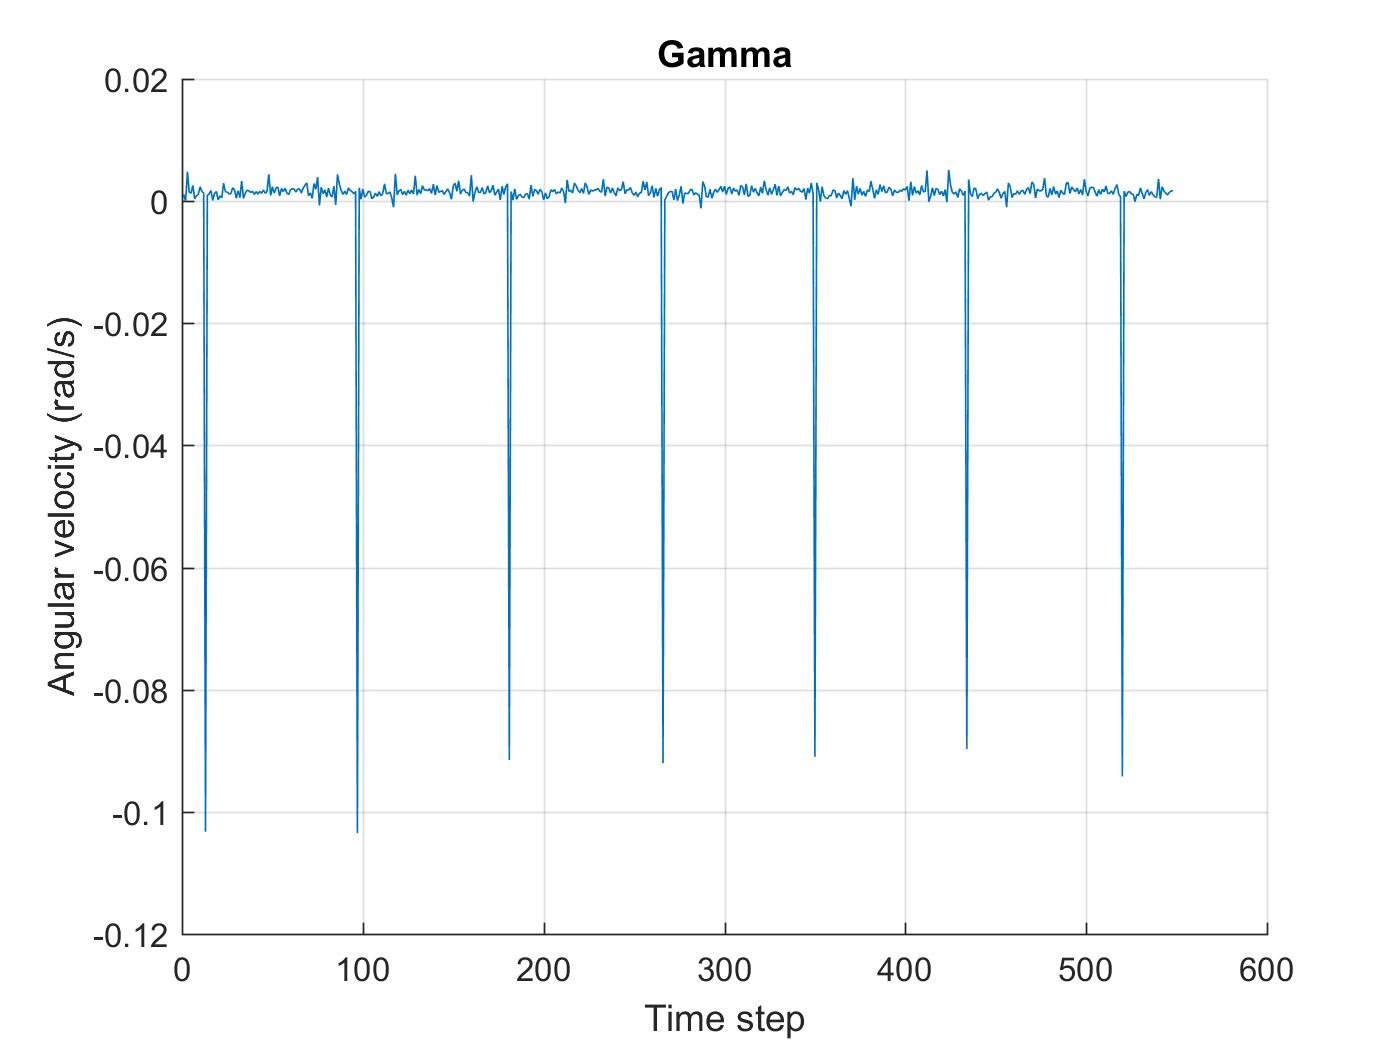
\includegraphics[width = 0.6\linewidth]{./figures/log3/gammaVsTime.jpg}
	\caption{log3:Gamma vs Time}
\end{figure}

\begin{figure}[H]
	\centering
	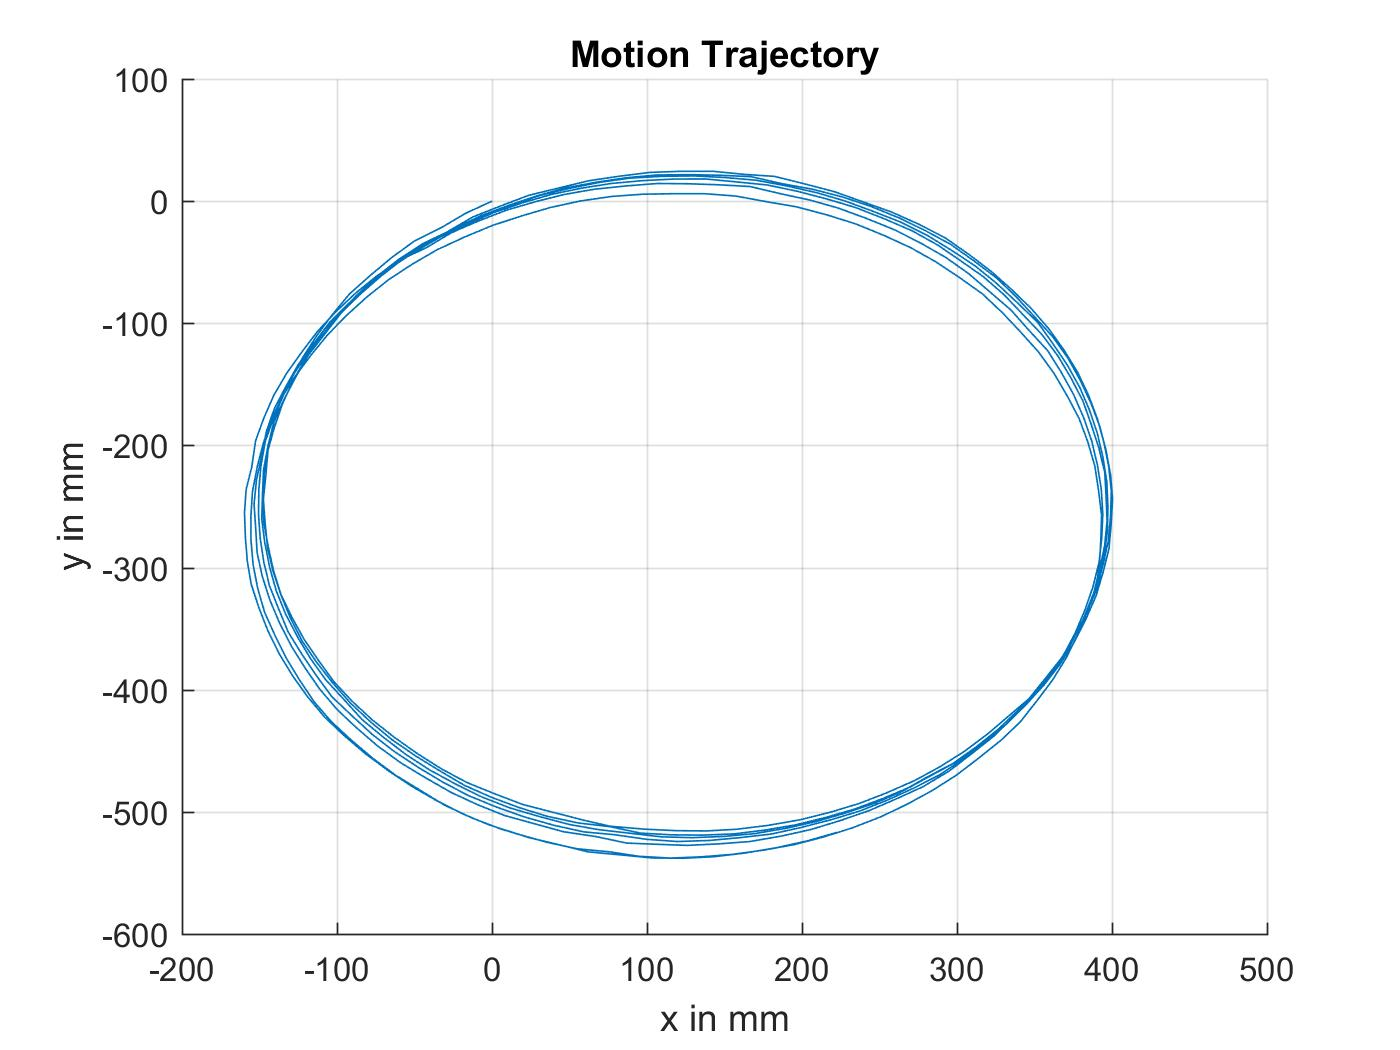
\includegraphics[width = 0.6\linewidth]{./figures/log3/motionTrajectory.jpg}
	\caption{log3:Motion Trajectory}
\end{figure}

\begin{figure}[H]
	\centering
	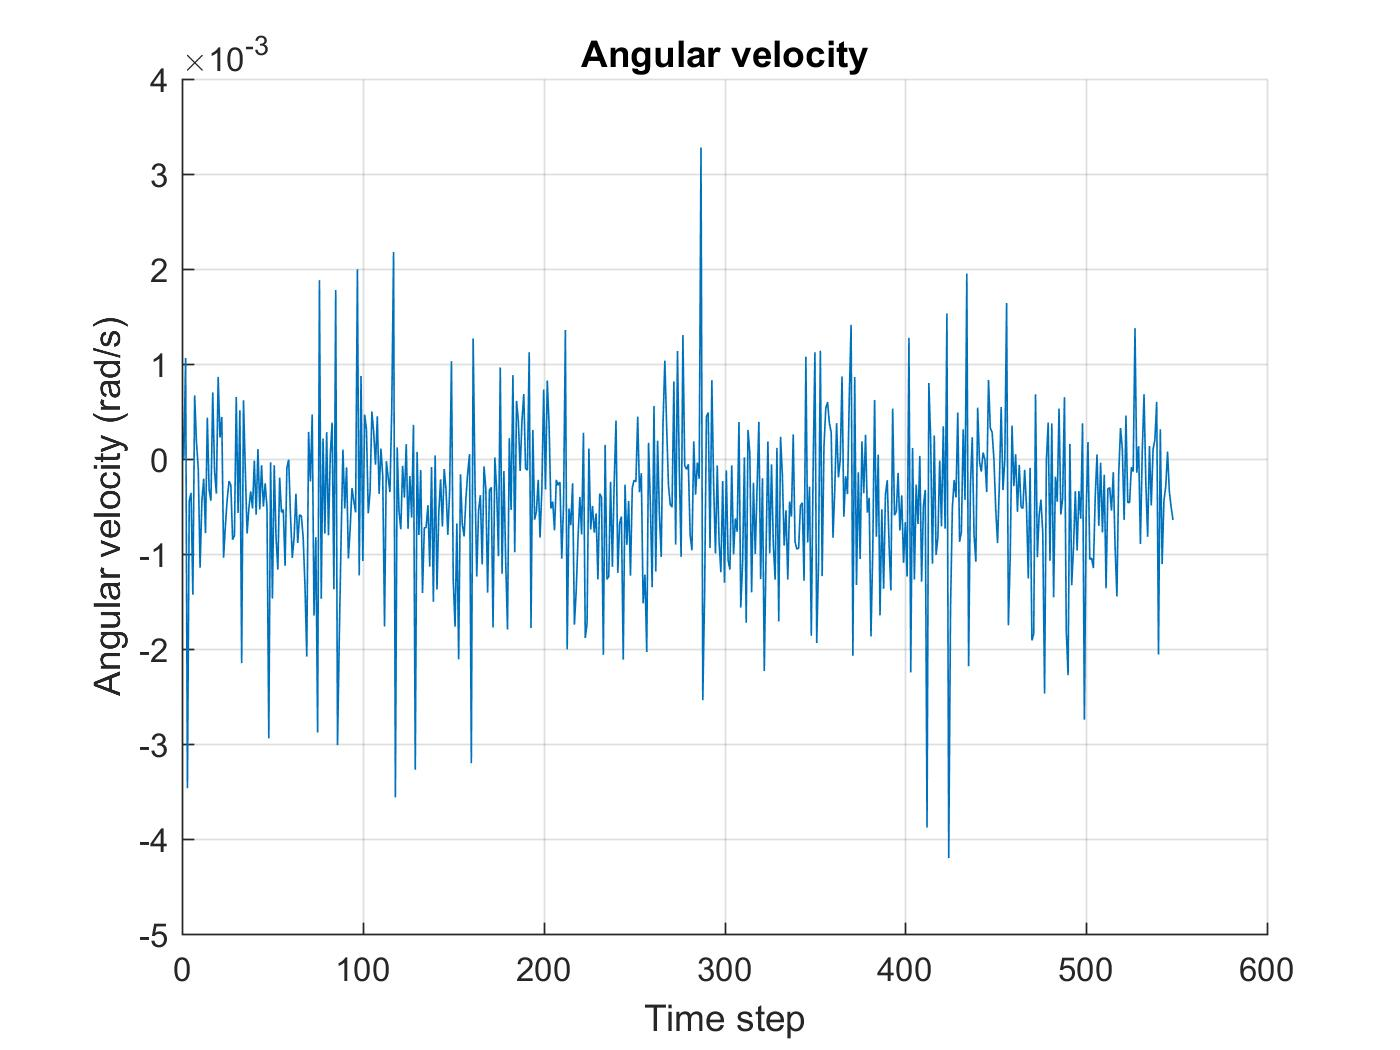
\includegraphics[width = 0.6\linewidth]{./figures/log3/omegaVsTime.jpg}
	\caption{log3:Omega vs Time}
\end{figure}

\begin{figure}[H]
	\centering
	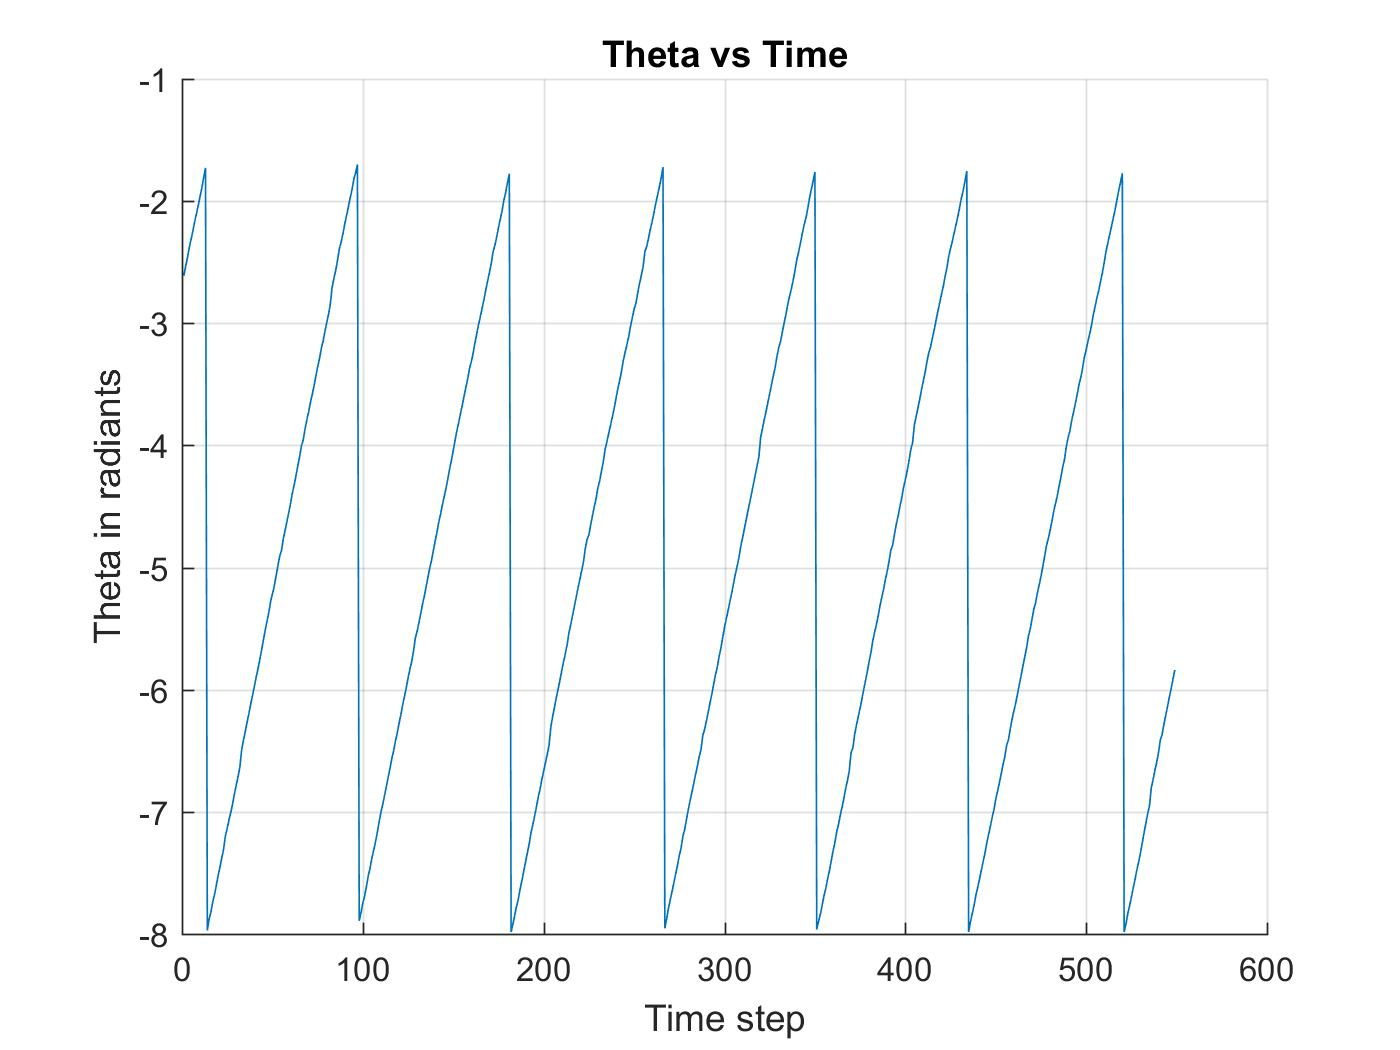
\includegraphics[width = 0.6\linewidth]{./figures/log3/thetaVsTime.jpg}
	\caption{log3:Theta vs Time}
\end{figure}

\begin{figure}[H]
	\centering
	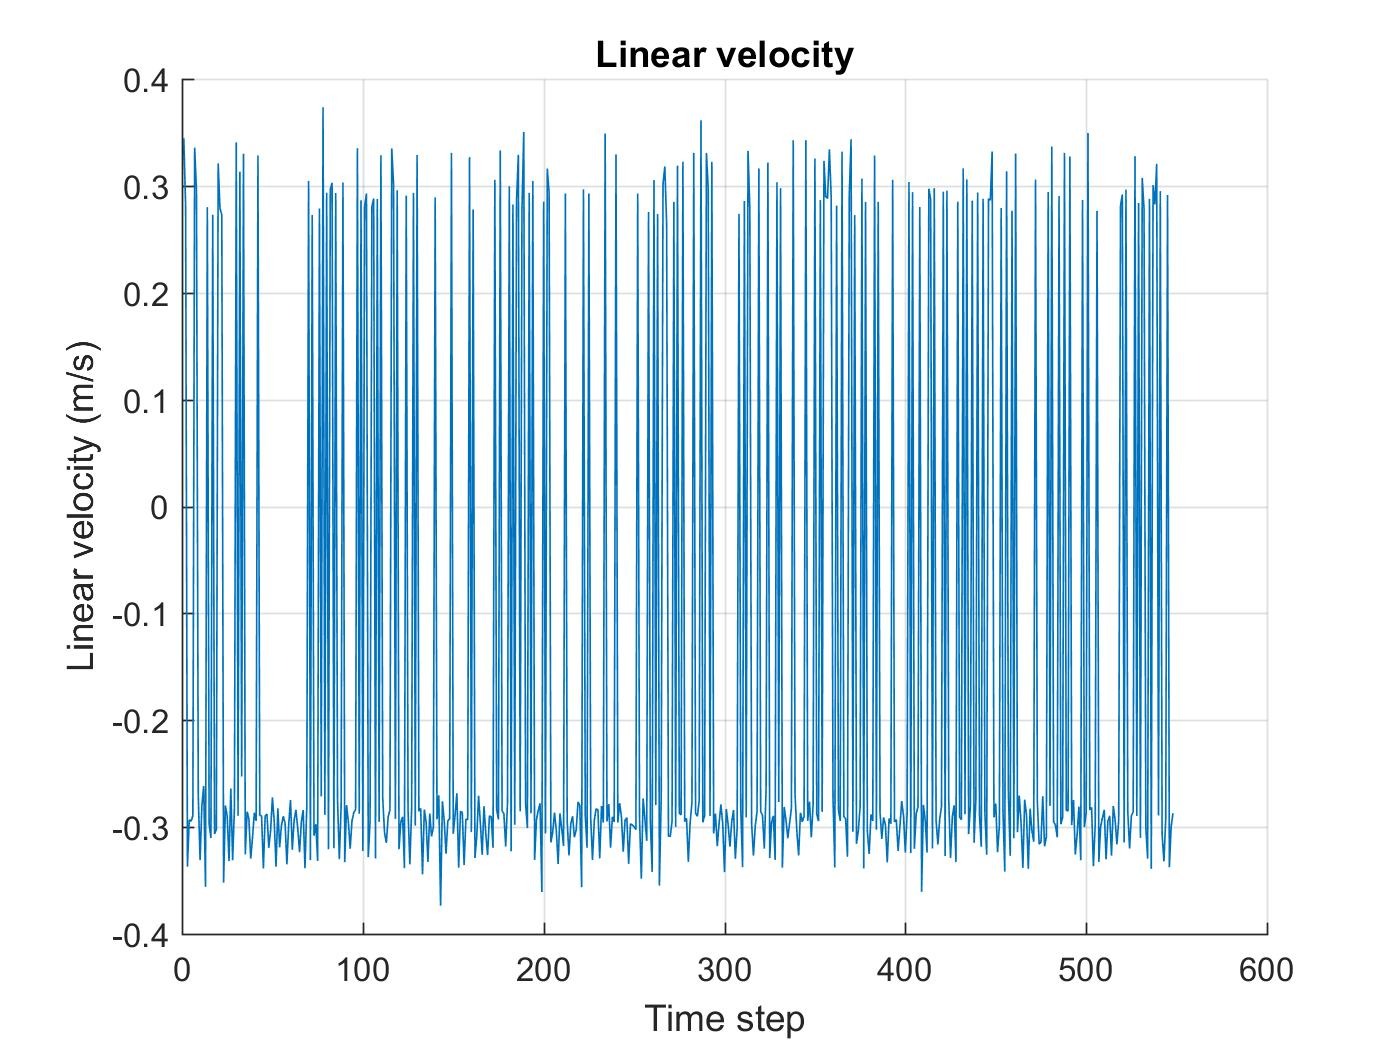
\includegraphics[width = 0.6\linewidth]{./figures/log3/vVsTime.jpg}
	\caption{log3:V vs Time}
\end{figure}

\begin{figure}[H]
	\centering
	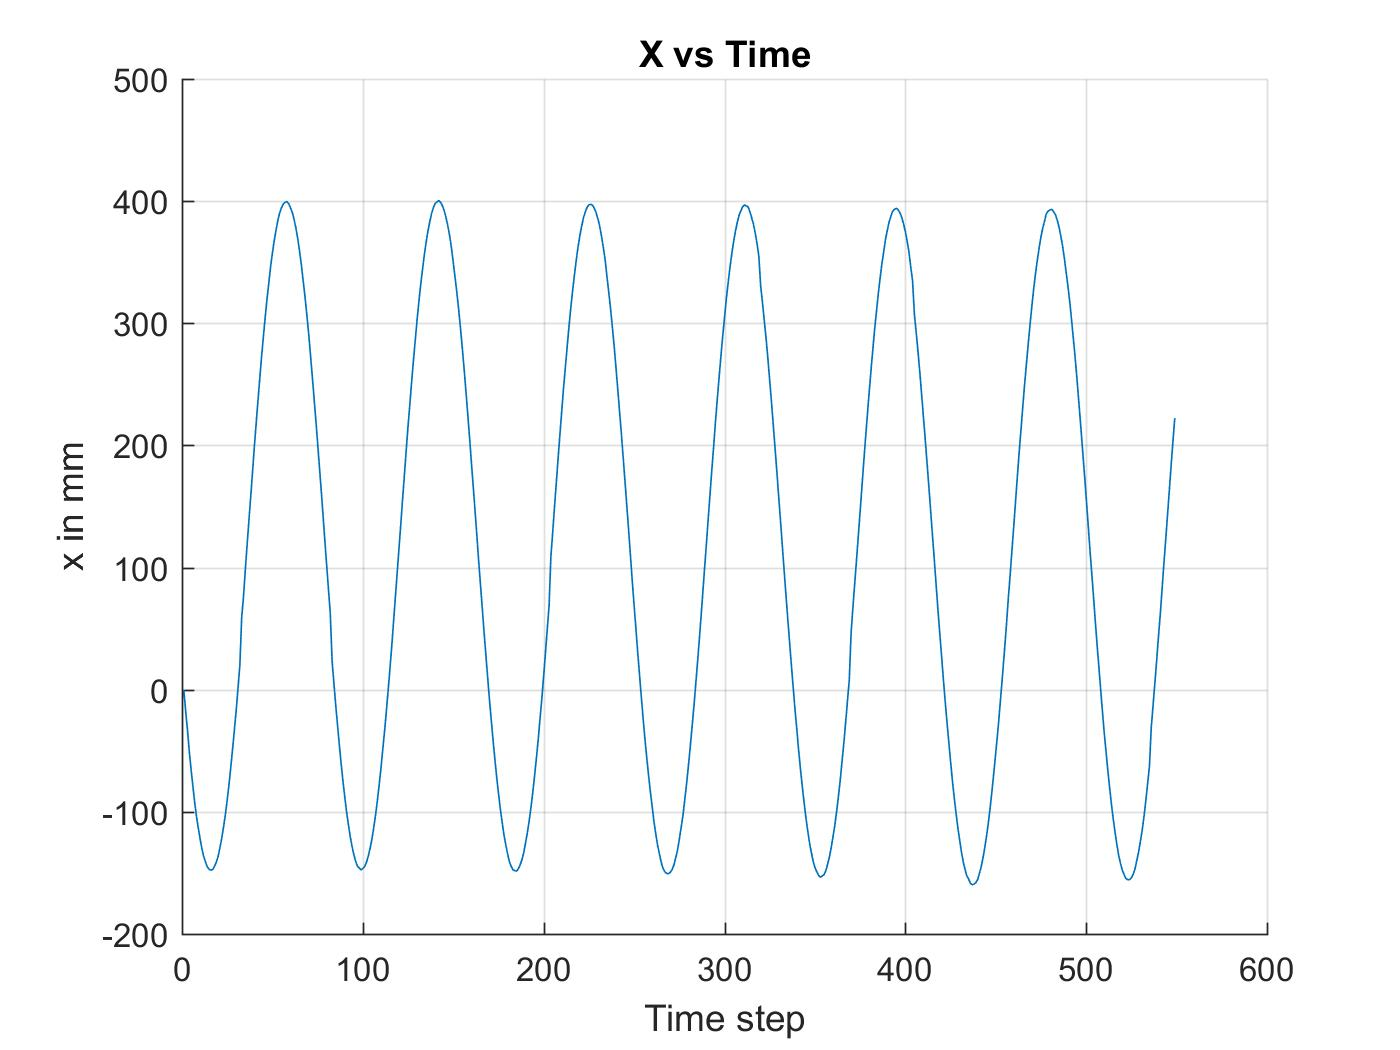
\includegraphics[width = 0.6\linewidth]{./figures/log3/xVsTime.jpg}
	\caption{log3:X vs Time}
\end{figure}

\begin{figure}[H]
	\centering
	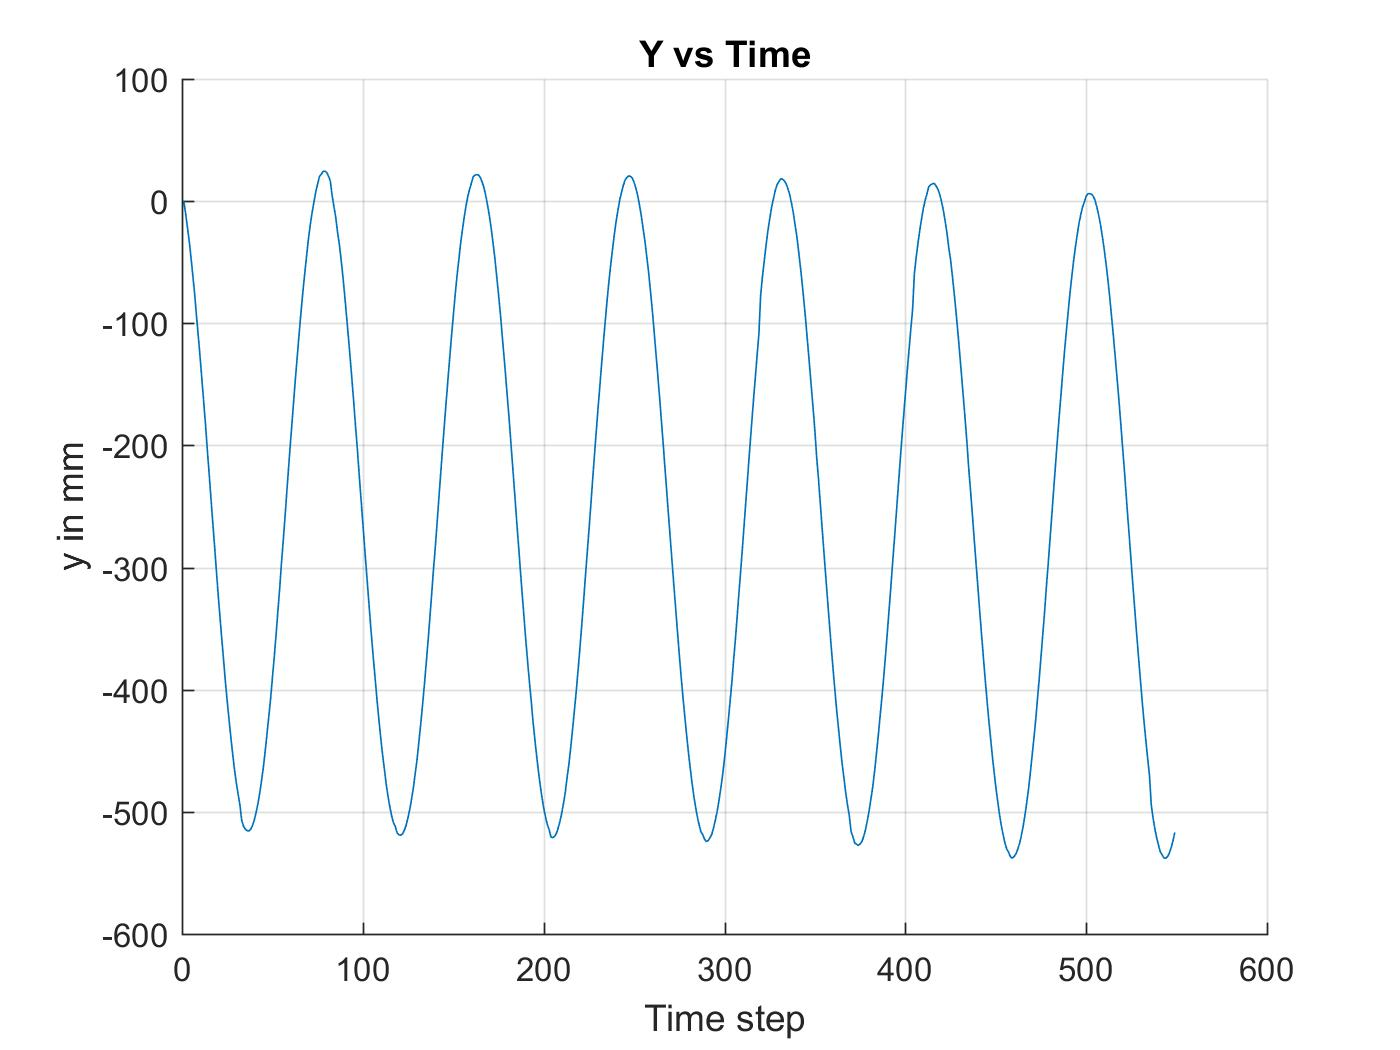
\includegraphics[width = 0.6\linewidth]{./figures/log3/yVsTime.jpg}
	\caption{log3:Y vs Time}
\end{figure}

%log 4
\begin{figure}[H]
	\centering
	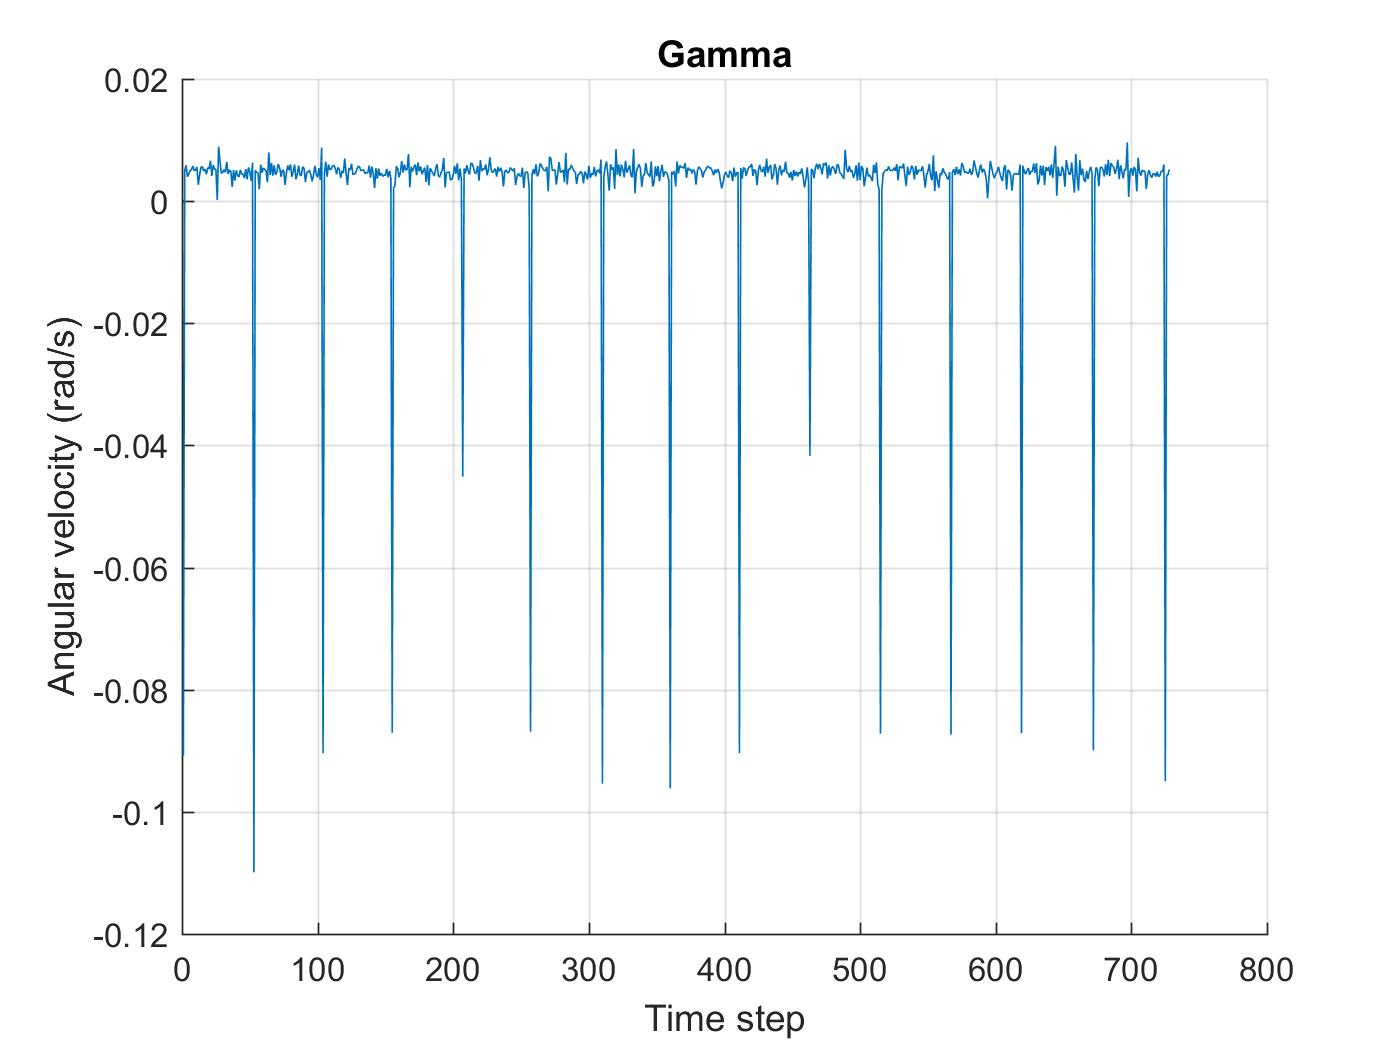
\includegraphics[width = 0.6\linewidth]{./figures/log4/gammaVsTime.jpg}
	\caption{log4:Gamma vs Time}
\end{figure}

\begin{figure}[H]
	\centering
	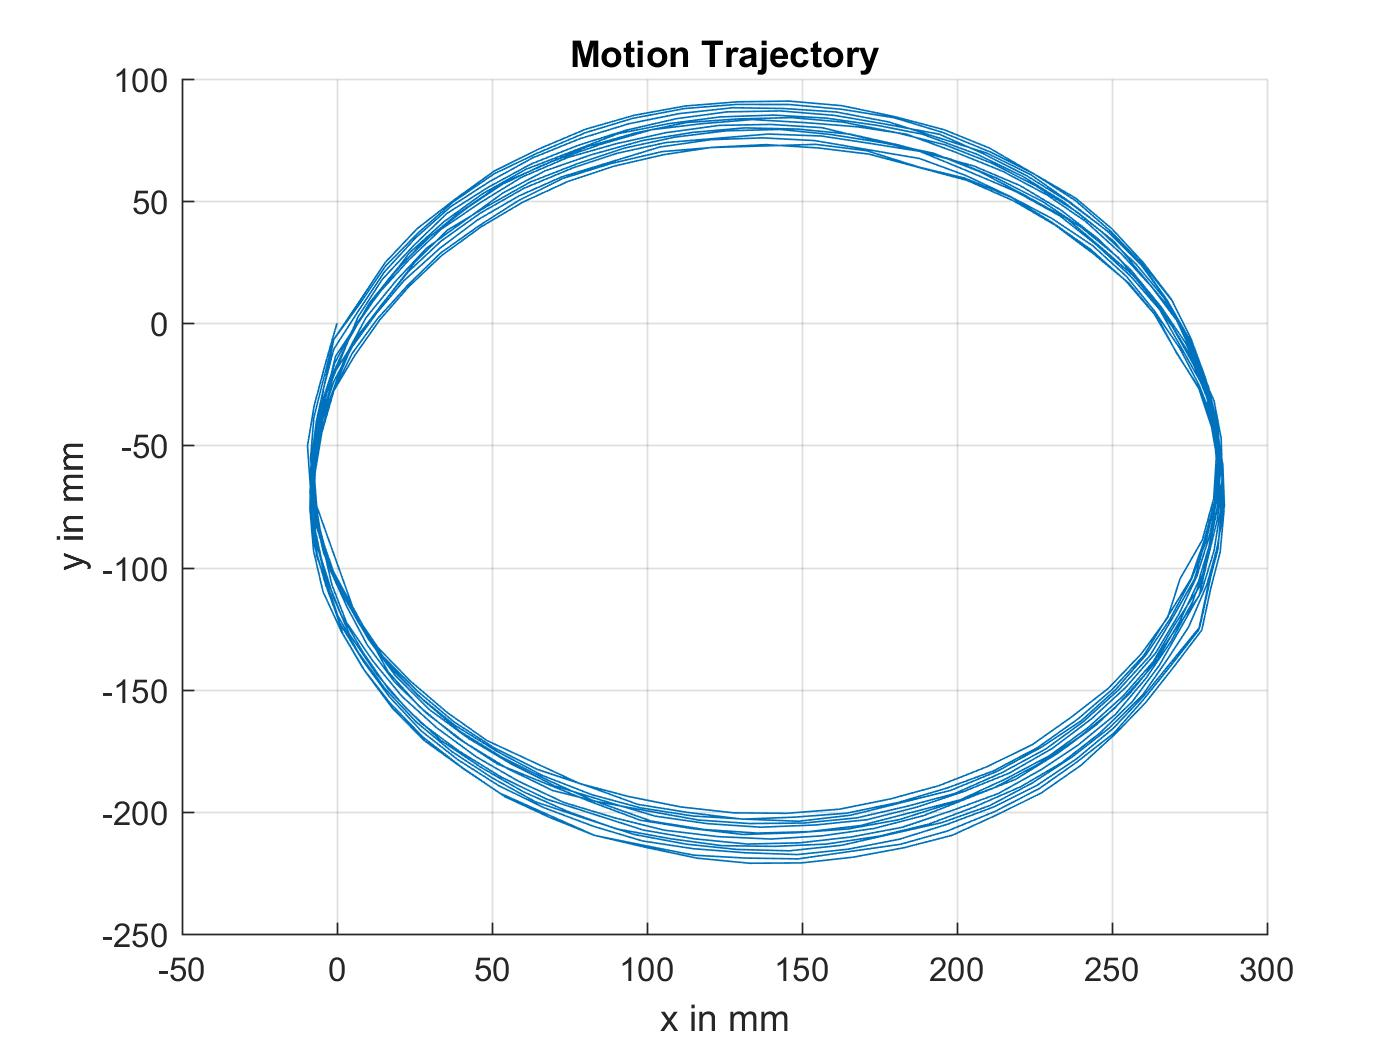
\includegraphics[width = 0.6\linewidth]{./figures/log4/motionTrajectory.jpg}
	\caption{log4:Motion Trajectory}
\end{figure}

\begin{figure}[H]
	\centering
	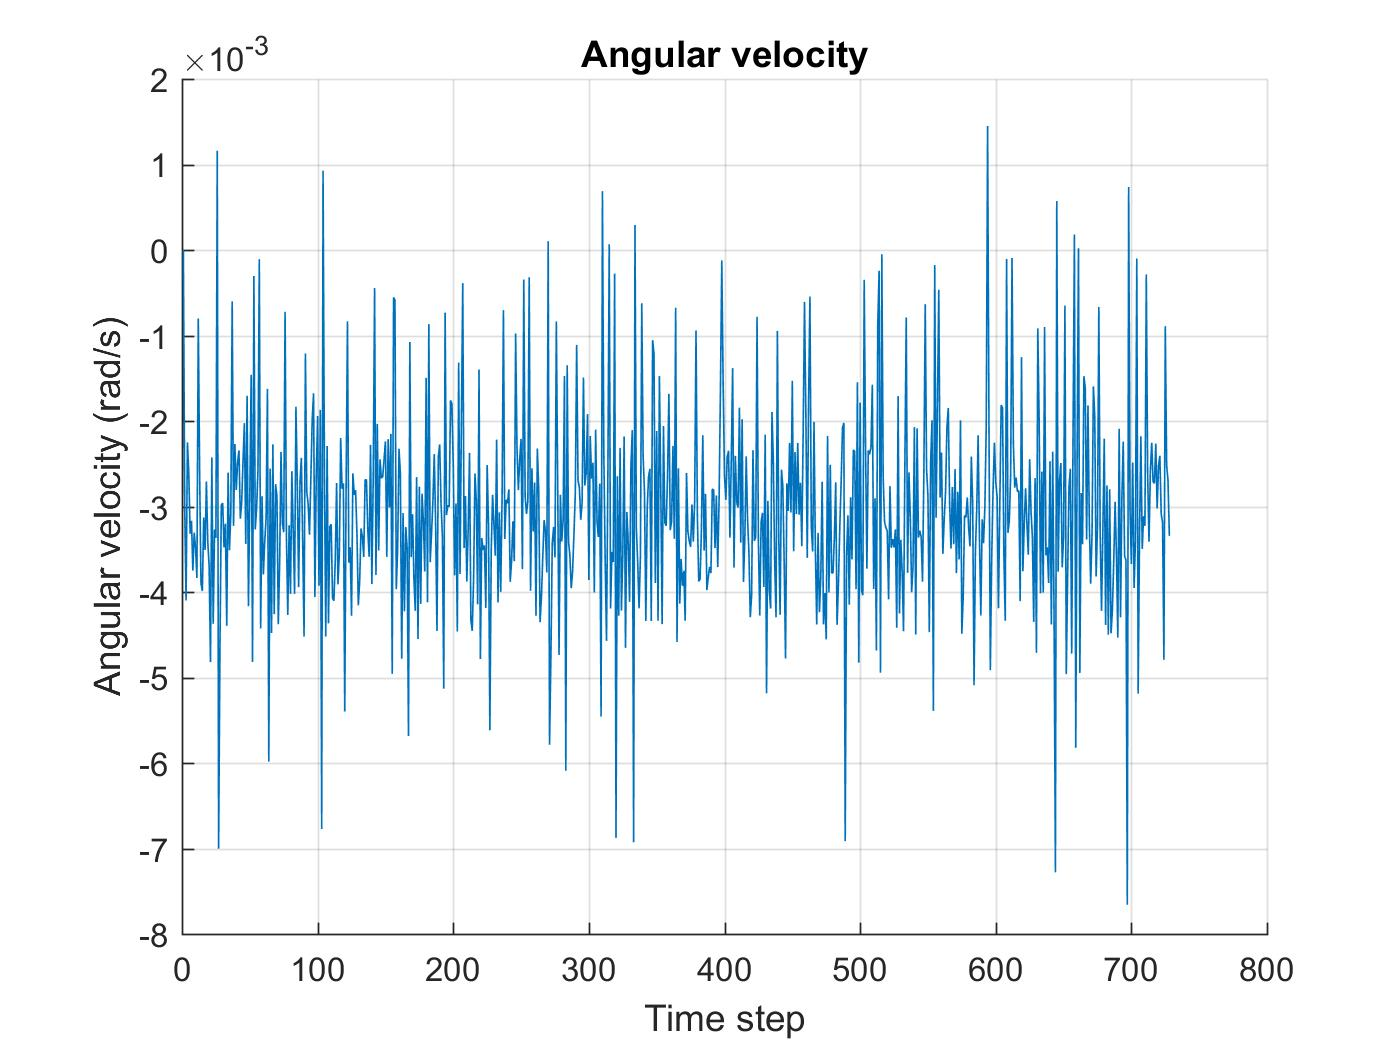
\includegraphics[width = 0.6\linewidth]{./figures/log4/omegaVsTime.jpg}
	\caption{log4:Omega vs Time}
\end{figure}

\begin{figure}[H]
	\centering
	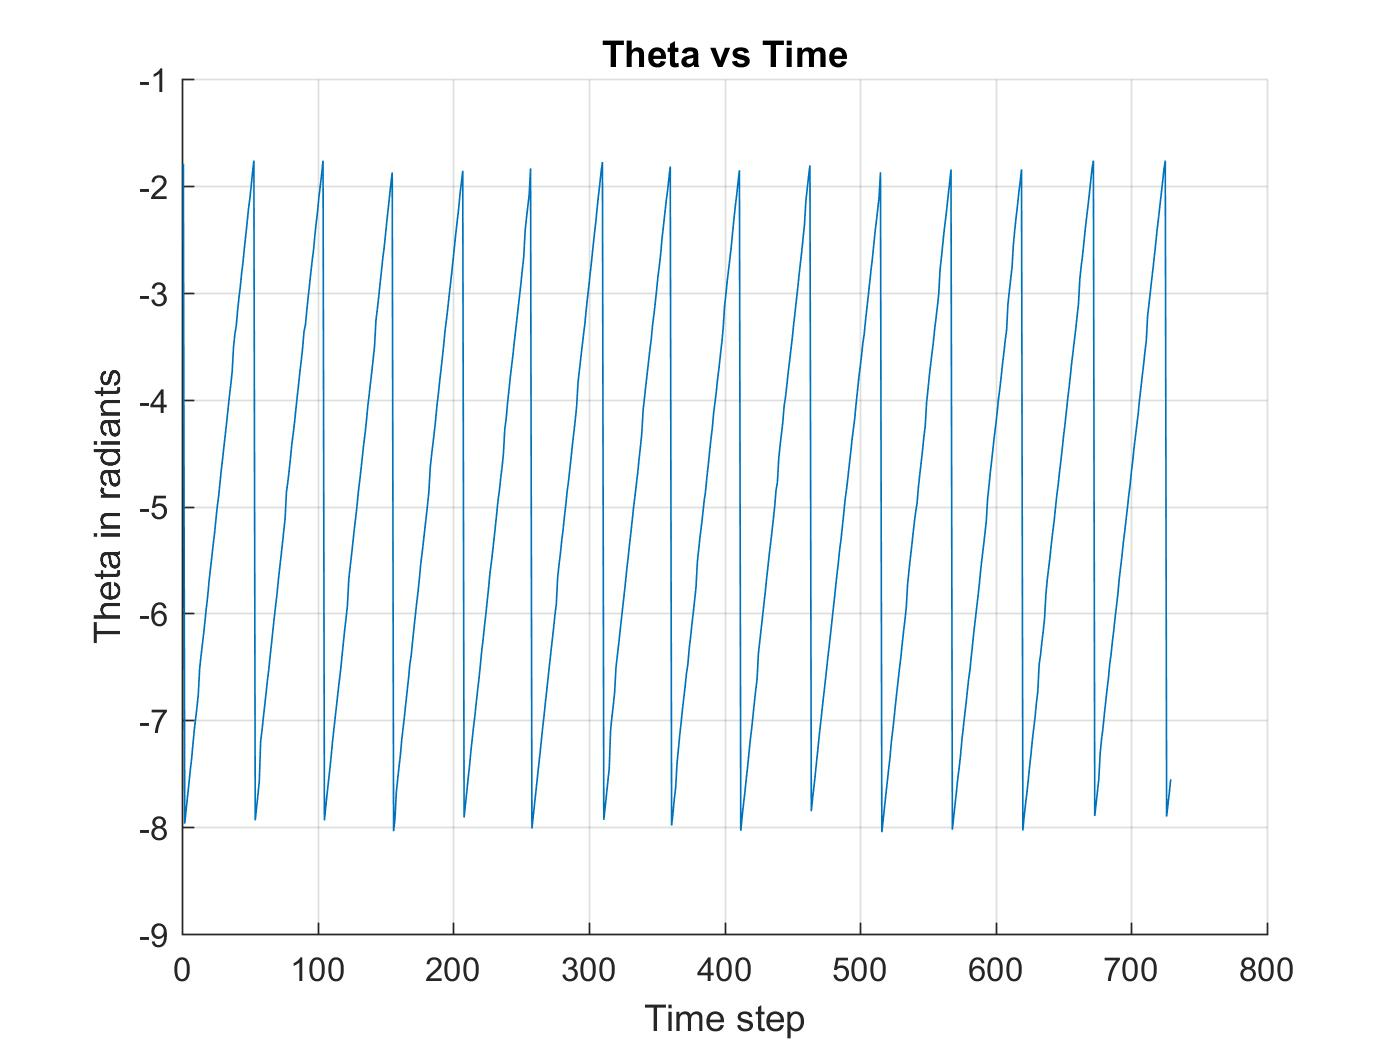
\includegraphics[width = 0.6\linewidth]{./figures/log4/thetaVsTime.jpg}
	\caption{log4:Theta vs Time}
\end{figure}

\begin{figure}[H]
	\centering
	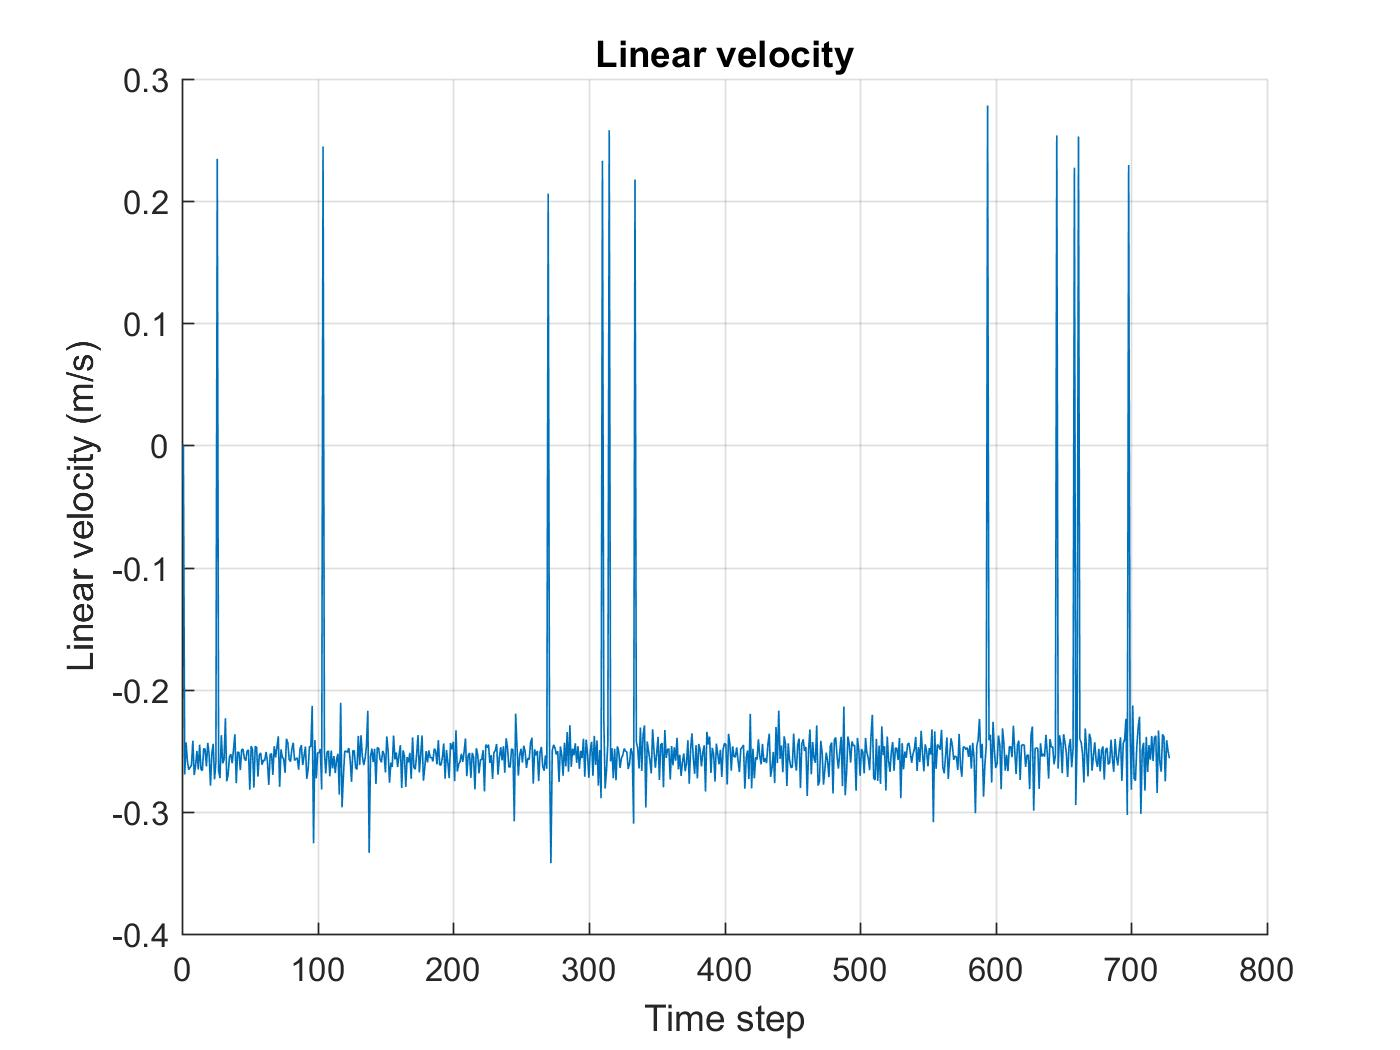
\includegraphics[width = 0.6\linewidth]{./figures/log4/vVsTime.jpg}
	\caption{log4:V vs Time}
\end{figure}

\begin{figure}[H]
	\centering
	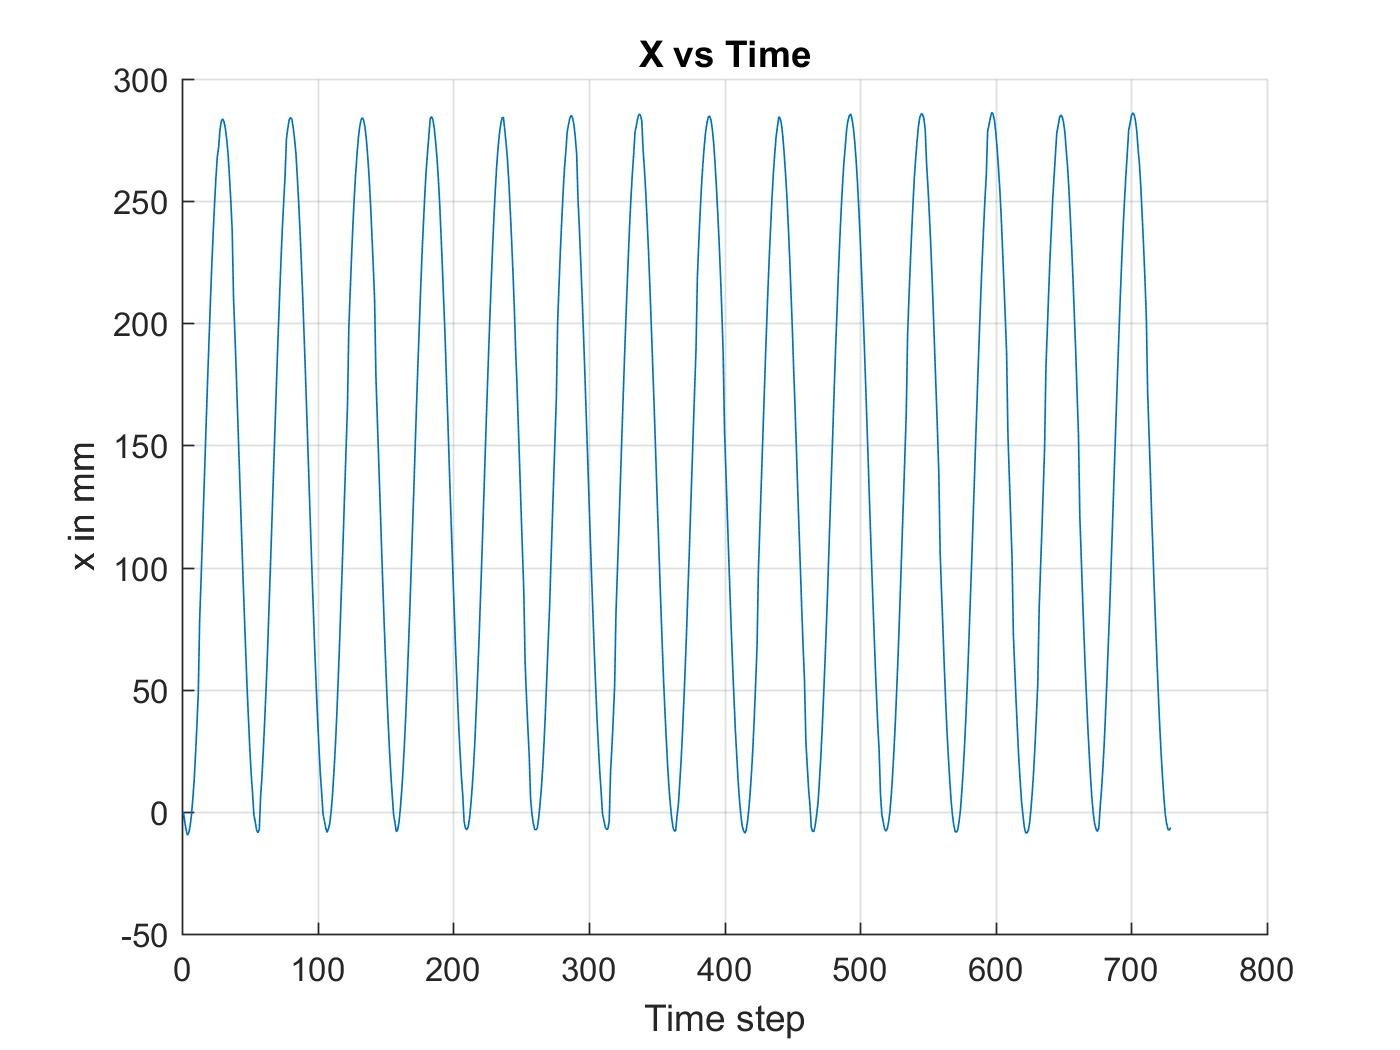
\includegraphics[width = 0.6\linewidth]{./figures/log4/xVsTime.jpg}
	\caption{log4:X vs Time}
\end{figure}

\begin{figure}[H]
	\centering
	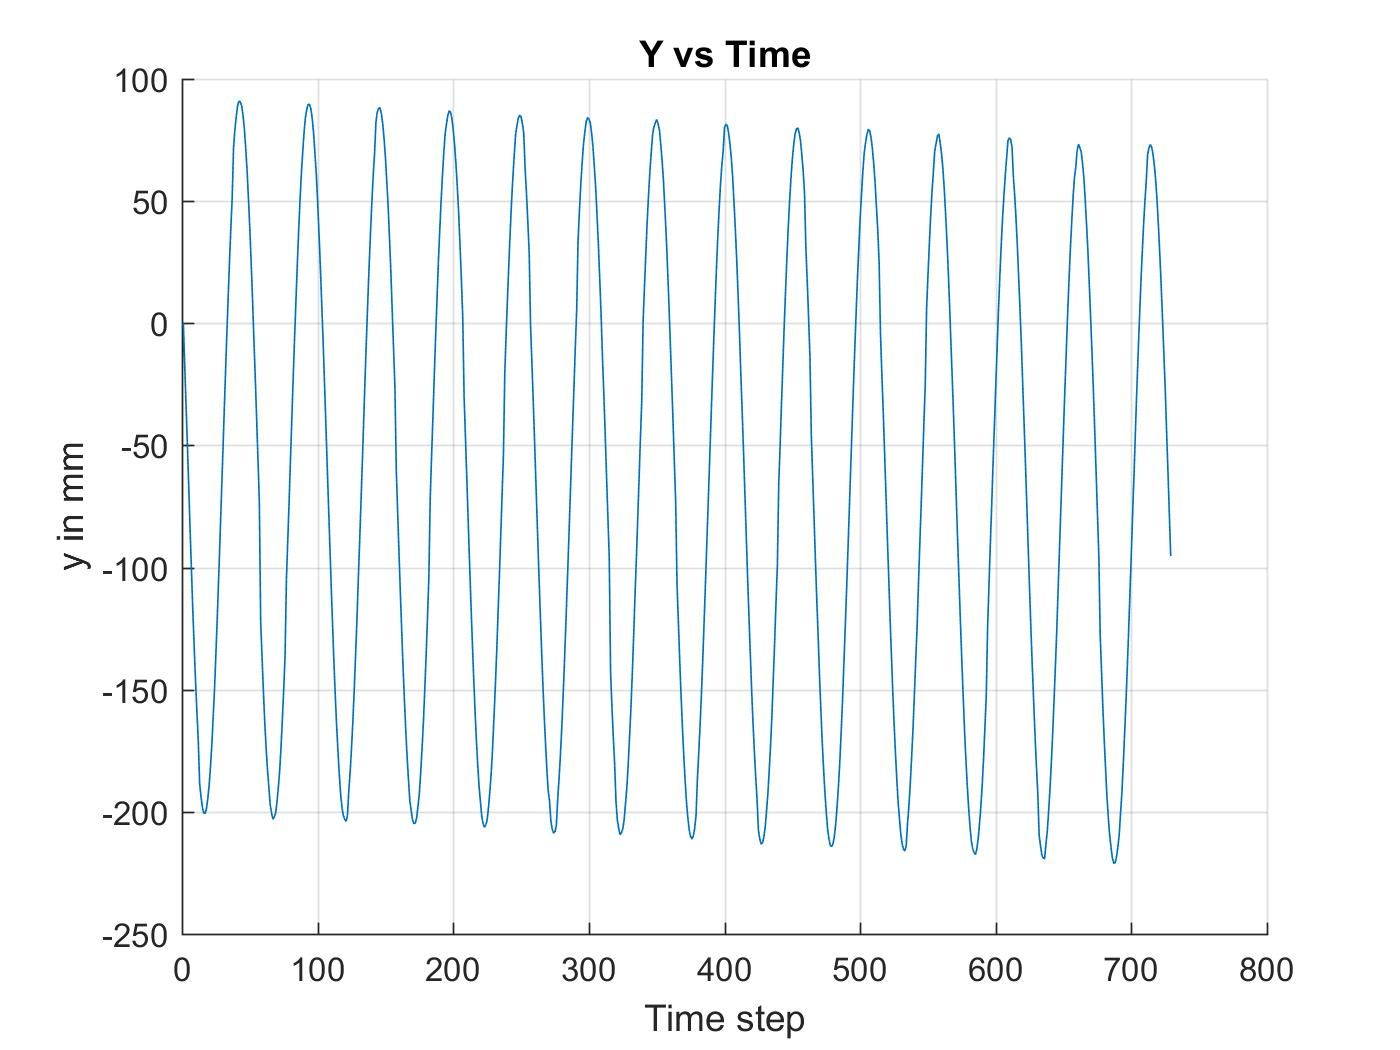
\includegraphics[width = 0.6\linewidth]{./figures/log4/yVsTime.jpg}
	\caption{log4:Y vs Time}
\end{figure}


\section{Source Code}
\subsection{Compute Alpha}
\lstinputlisting{computeAlpha.m}
\subsection{Anaylize Motion Log}
\lstinputlisting{analyzeMotionLog.m}
\end{appendix}

\end{document}